\PassOptionsToPackage{french,english,dutch}{babel}
\documentclass[twoside]{extreport}

\usepackage{inbo_report}
\codesize{\footnotesize}




\title{Het voorkomen van de Vossenlintworm (\emph{Echinococcus multilocularis})
in de Muskusrat (\emph{Ondatra zibethicus}) in Vlaanderen.}
\subtitle{Screening op de aanwezigheid van cysten in muskusratten gevangen door
VMM in kader van bestrijding.}
\author{Emma Cartuyvels, Kristof Baert, Koen Van Den Berge, Filip Berlengee, Jan Stuyck}

\reportnumber{doi.org/10.21436/inbor.17747724}




% Alter some LaTeX defaults for better treatment of figures:
% See p.105 of "TeX Unbound" for suggested values.
% See pp. 199-200 of Lamport's "LaTeX" book for details.
%   General parameters, for ALL pages:
\renewcommand{\topfraction}{0.9}	% max fraction of floats at top
\renewcommand{\bottomfraction}{0.8}	% max fraction of floats at bottom
%   Parameters for TEXT pages (not float pages):
\setcounter{topnumber}{2}
\setcounter{bottomnumber}{2}
\setcounter{totalnumber}{4}     % 2 may work better
\setcounter{dbltopnumber}{2}    % for 2-column pages
\renewcommand{\dbltopfraction}{0.9}	% fit big float above 2-col. text
\renewcommand{\textfraction}{0.07}	% allow minimal text w. figs
%   Parameters for FLOAT pages (not text pages):
\renewcommand{\floatpagefraction}{0.7}	% require fuller float pages
% N.B.: floatpagefraction MUST be less than topfraction !!
\renewcommand{\dblfloatpagefraction}{0.7}	% require fuller float pages

\let\BeginKnitrBlock\begin \let\EndKnitrBlock\end
\begin{document}
\maketitle
\pagenumbering{arabic}


%starttoc

\clearpage

\phantomsection
\setcounter{tocdepth}{3}
\tableofcontents
\addcontentsline{toc}{chapter}{\contentsname}

\clearpage

\phantomsection
\listoffigures
\addcontentsline{toc}{chapter}{\listfigurename}
\vspace{34pt}

\phantomsection
\listoftables
\addcontentsline{toc}{chapter}{\listtablename}

\clearpage

%endtoc

\chapter*{Dankwoord}\label{dankwoord}
\addcontentsline{toc}{chapter}{Dankwoord}

Dit onderzoek werd uitgevoerd in opdracht van de Vlaamse
Milieumaatschappij (VMM), Afdeling Operationeel Waterbeheer. Het was
enkel te realiseren door hun bereidwilligheid om alle gevangen
muskusratten ter beschikking te stellen voor dit onderzoek. Door het
continue en semi-gebiedsdekkende karakter van hun bestrijdingswerk,
waarbij steeds een nultolerantie wordt gehanteerd en een onafhankelijke
controlemeting garant staat voor de kwaliteit van het geleverde
resultaat, vormen deze gegevens het essentiële vertrekpunt van alle
verdere onderzoek. Enkel op deze wijze konden we beschikken over de
basisgegevens met betrekking tot het voorkomen van muskusratten in
Vlaanderen en de grensgebieden met Wallonië en Frankrijk.

Met dank aan Lode De Beck en Marc Pollet voor het kritisch nalezen van
een eerdere versie van dit rapport.

\chapter*{Samenvatting}\label{samenvatting}
\addcontentsline{toc}{chapter}{Samenvatting}

Sinds 1994 worden in Vlaanderen (en net over de grens) gevangen
muskusratten (\emph{Ondatra zibethicus}) gedissecteerd om hun ecologie
te doorgronden. Tijdens deze dissecties vielen de grote hoeveelheden
parasieten in de buikholte van onderzochte dieren op, waarbij
kattenlintworm (\emph{Taenia taeniaformes}) veruit het meest voorkomend
was.

In 2008 werd de eerste muskusrat besmet met vossenlintworm
(\emph{Echinococcus multilocularis} of EM) gevonden, afkomstig uit
Lessines (prov. Henegouwen, Wallonië), nabij de gewestgrens. Vanaf 2009
werden daarom alle muskusratten, die door VMM-bestrijders werden
gevangen in Vlaanderen, Wallonië of Frankrijk, ingezameld en bij het
INBO onderzocht.

Bij een visuele controle van de lever van 15.948 muskusratten uit de
periode 2008 tot 2017 werden 203 met EM besmette dieren aangetroffen
(1,30\%). In Vlaanderen ging het om 82 besmette exemplaren van de 9.425
(0,87\%). Terwijl we in het grootste deel van Vlaanderen geen
aanwijzingen hebben gevonden voor de aanwezigheid van deze parasiet,
hebben we voldoende bewijs van het voorkomen van EM in het
gewestgrensgebied van zowel Schelde-, Dender-, Zenne-, Dijle- als
Maasbekken.

De verwachte uitbreiding van vossenlintworm over heel Vlaanderen vanuit
Wallonië heeft dus niet plaatsgevonden. Wij argumenteren dat het laag
houden van de muskusrattenpopulatie hierin mogelijk een belangrijke rol
heeft gespeeld.

\chapter*{Aanbevelingen voor beheer en/of
beleid}\label{aanbevelingen-voor-beheer-enof-beleid}
\addcontentsline{toc}{chapter}{Aanbevelingen voor beheer en/of beleid}

Volgens de meest recente vaststellingen komt vossenlintworm weinig voor
bij vossen in Vlaanderen
\citep{vervaeke2012vossenlintworm, vervaeke2014geen, vervaeke2014bis}.
Ons onderzoek toont aan dat ook bij muskusratten, een van de
tussengastheren van de parasiet, de prevalentie in Vlaanderen zeer laag
is. Wij vermoeden dat de lage populatiedichtheid van de muskusrat,
dankzij de toegepaste bestrijding, een grote rol speelt in de geringe
lintwormprevalentie. Door haar verhoogde gevoeligheid voor EM, ten
opzichte van de natuurlijk aanwezige tussengastheren, speelt de
muskusrat immers een grote potentiële rol in het vervolledigen van de
vossenlintwormcyclus in Vlaanderen. Het blijven inzetten op het zo sterk
mogelijk beperken van de muskusrattenpopulatie in Vlaanderen is daarom
een belangrijke aanbeveling. Gezien de lage prevalentie worden sommige
maatregelen die in het buitenland genomen worden, zoals ontwormen van
vossen met behulp van lokaas of de permanente screening van mensen
actief in de bos-, land- en tuinbouw, in Vlaanderen minder (of niet)
zinvol geacht. Uit wetenschappelijk onderzoek blijkt ook dat het bejagen
van vossen geen oplossing biedt maar integendeel contraproductief kan
werken in het tegengaan van de verspreiding van EM
\citep{craig2017echinococcosis, comte2017echinococcus}. Wij bevelen
daarom aan in te zetten op sensibilisatie van de bevolking en meer
specifiek op volgende punten:

\begin{itemize}
\tightlist
\item
  Het grondig wassen van groenten en laaggroeiend fruit vooraleer het te
  consumeren.
\item
  Het toepassen van elementaire hygiëne-maatregelen (handen wassen voor
  het eten) na buiten-activiteiten.
\item
  Het regelmatig ontwormen van honden met ontwormingsmiddelen op basis
  van praziquantel, zeker wanneer ze regelmatig knaagdieren opeten en/of
  recent naar voor EM endemisch gebied (Ardennen, Noordoost-Frankrijk,
  Zuid-Duitsland, Zwitserland of Alpien Oostenrijk) zijn geweest.
\item
  Er een goede hygiëne op nahouden in het omgaan met honden.
\end{itemize}

\chapter*{English abstract}\label{english-abstract}
\addcontentsline{toc}{chapter}{English abstract}

Since 1994, muskrats (\emph{Ondatra zibethicus}) caught in Flanders (or
just across the border) have been dissected with the aim of
understanding their ecology. Whilst doing so a large number of parasites
were observed in the abdomen of the dissected animals, most notably
\emph{Taenia taeniaformes}.

In 2008 a first individual infected with fox tapeworm
(\emph{Echinococcus multilocularis}) was found, caught just across the
regional border in Wallonia. Hence, from 2009 onwards all muskrats
caught in Flanders, Wallonia and France by pest controllers of the
Flanders Environment Agency (VMM) were collected and dissected with the
aim of understanding the prevalence of this parasite.

Visual examination of the livers of 15.948 muskrats caught between 2008
and 2017 revealed 203 infected animals. Regionally we found 82 infected
animals out of 9.425 (0,87\%) in Flanders. All of the infected animals
were found in municipalities bordering the Flemish-Walloon border.

Although EM infection was expected to spread northward from Wallonia to
Flanders, this was not observed in the dissected muskrats. Here we argue
that keeping muskrat populations low through extensive culling programs
may have aided in stopping this spread.

\chapter{Inleiding en
onderzoekskader}\label{inleiding-en-onderzoekskader}

\section{Inleiding}\label{inleiding}

In 1992 werd een onderzoeksproject opgestart betreffende de Vlaamse
muskusratbestrijding aan het toenmalige Centrum voor Landbouwkundig
Onderzoek (CLO). Bij dit onderzoek werden o.a. gevangen muskusratten
(\emph{Ondatra zibethicus} Linnaeus 1766) gedissecteerd om de
voortplantingsgegevens bij de weggevangen dieren te onderzoeken. Hierbij
viel de veelvuldige aanwezigheid van endoparasieten bij de onderzochte
dieren op. Vooral het voorkomen van lintwormcysten in de lever was in
sommige gevallen spectaculair en verdiende verdere aandacht. Enerzijds
zouden ze een oorzaak van natuurlijke mortaliteit in de
muskusratpopulatie kunnen betekenen, anderzijds zouden ze belangrijk
kunnen zijn voor eind- of tussengastheren, of mogelijk een gevaar voor
de rattenvangers inhouden.

Vanaf 1994 werd daarom bij de dissectie van muskusratten steeds de
aanwezigheid van lintwormen of cestoden opgevolgd. Al snel werd
duidelijk dat er in de onderzochte muskusratten hoofdzakelijk cysten van
de kattenlintworm, \emph{Taenia taeniaeformis} (Fig.
\ref{fig:Muskusratlever}), in de lever worden aangetroffen, maar ook
\emph{T. martis} en \emph{T. crassiceps} werden occasioneel in de
buikholte teruggevonden. De opvolging van de aanwezigheid van cysten in
de lever werd daarom een constante in het muskusrattenonderzoek.




\begin{figure}

{\centering 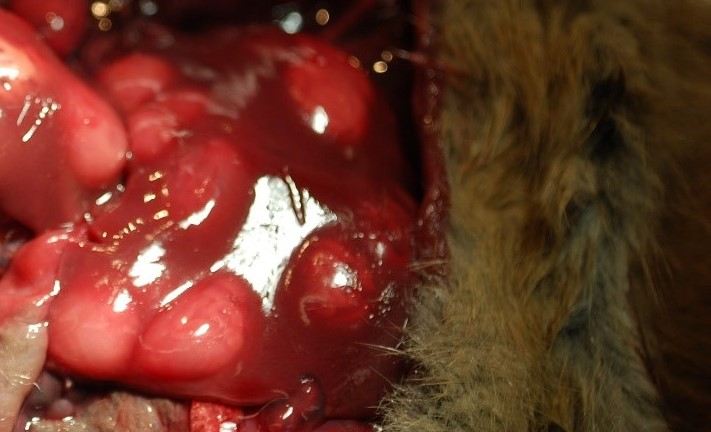
\includegraphics[width=0.6\linewidth]{Taenia_cysten} 

}

\caption{Muskusratlever met cysten van \emph{Taenia
taeniaeformis}.}\label{fig:Muskusratlever}
\end{figure}

In Wallonië werden in 2003-2004, 192 van de 1718 onderzochte
muskusratten positief bevonden voor vossenlintworm (\emph{Echinococcus
multilocularis} (EM)) \citep{hanosset2008echinococcus}. Ook in
Nederland, Frankrijk en Duitsland werden al vóór 2008 positieve
muskusratten gevonden \citep{oksanen2016geographical}. In 2008 werd door
het INBO een eerste vaststelling gedaan van EM in één muskusrat uit
Ghoy, deelgemeente van Lessines in de provincie Henegouwen. Het besmette
dier maakte deel uit van 182 muskusratten die werden gevangen tijdens
een controlevangst in het kader van het Euregio-project Cartora. Dit
project hield een samenwerkingsverband in tussen de Vlaamse, Waalse en
Franse muskusratbestrijdingsorganisaties werkzaam in de grensstreek met
Vlaanderen, tussen De Panne (West-Vlaanderen) en Brakel
(Oost-Vlaanderen). Hierbij werden occasioneel door VMM ook muskusratten
in de Franse en Waalse grensgemeentes gevangen. Vanaf dat moment werden
alle gevangen muskusratten op een meer systematische wijze door VMM
ingezameld en ter beschikking gesteld aan het INBO voor verder
onderzoek.

\section{Waarom EM-onderzoek bij de
Muskusrat?}\label{waarom-em-onderzoek-bij-de-muskusrat}

Onderzoek naar EM gebeurt vooral in het kader van de volksgezondheid. De
mens kan immers besmet geraken met de eieren van deze parasiet. Wanneer
deze zich in de lever ontwikkelen, met kans op uitzaaiing naar andere
plaatsen in het lichaam, kan dit op lange termijn leiden tot een
levensbedreigende infectie: alveolaire echinococcose (AE). Door de
sterke toename van de vos in Europa op het einde van vorige eeuw
\citep{vandenberge2003vos, vandenberge2013stadsvos}, groeide ook de
bezorgdheid voor een uitbreiding van deze ernstige parasitose
\citep{eckert2001oie, eckert2004biological} en werd er steeds meer
aandacht aan besteed en onderzoek naar uitgevoerd.

De meest voor de hand liggende monitoring van het voorkomen van EM
gebeurt door het onderzoeken van de vossenpopulatie. De vos is immers
eindgastheer, drager van de volwassen lintworm en zodoende potentiële
verspreider van de voor de mens en knaagdieren infectieuze EM-eieren.
Verschillende technieken kunnen hierbij worden gebruikt, zoals het
opsporen van de adulte lintwormen in de dunne darm, of van
lintwormeitjes in de inhoud van het rectum of in uitwerpselen die in het
veld werden gevonden. Ook genetische technieken kunnen hierbij gebruikt
worden. Het ANB volgde gespreid over de periode van 2011 tot 2014 de
vossenlintworm in de Vlaamse vossenpopulatie op
\citep{vervaeke2012vossenlintworm, vervaeke2014geen, vervaeke2014bis}.

Het statistisch correct samplen van de vossenpopulatie is echter
bijzonder moeilijk \citep{tackmann1998spatial, conraths2003statistics}.
Aanvullend aan het bemonsteren van vossenpopulaties wordt daarom ook
aandacht besteed aan het onderzoek van de knaagdieren, in het bijzonder
van woelmuissoorten (onderfamilie Arvicolinae), die de rol van
tussengastheer vervullen \citep{umhang2013nutrias}. In de kerngebieden
met een hoge EM-prevalentie wordt vooral de veldmuis (\emph{Microtus
arvalis}) als tussengastheer van EM aangeduid. Er werd ook een verband
gelegd tussen gebieden met een hoge densiteit aan deze woelmuizen en het
aantal besmette vossen/aantal klinische patiënten. In gebieden met de
nodige klimatologische kenmerken en een voldoende hoge
muskusratdensiteit, zou de muskusrat -- eveneens een woelmuissoort --
echter de rol van de kleinere woelmuizen kunnen versterken of zelfs
overnemen, met een toename van het areaal en de besmettingsgraad in het
gebied tot gevolg. Specifiek levert onderzoek naar EM in muskusratten
volgende voordelen:

\begin{itemize}
\tightlist
\item
  Muskusratten nemen de infectieuze eieren op via gecontamineerd voedsel
  en vegetatie. De mate waarin deze knaagdiersoort besmet is, geeft een
  indicatie voor de aanwezigheid van infectieuze ei-stadia in de
  omgeving en dus van het potentiële risico voor de mens. Ze kan
  beschouwd worden als bioindicator voor de aanwezigheid van EM in
  nieuwe gebieden \citep{reperant2009rodents, umhang2013nutrias}. De
  muskusrat vertoont bovendien een grotere kans op infectie dan de van
  nature aanwezige tussengastheren en kan hierdoor zeer goed als
  sentinel- of verklikkerspecies \footnote{Sentinel- of
    verklikkerspecies zijn soorten die gebruikt worden om te waarschuwen
    voor bepaalde gevaren voor mensen zoals gassen, milieuvervuiling,
    infectieziektes of toxines. Deze soorten worden meer blootgesteld of
    zijn gevoeliger aan het specifieke gevaar, waardoor ze er eerder
    symptomen van vertonen en zo kunnen mensen die zich in dezelfde
    omgeving bevinden zich tijdig in veiligheid brengen.} fungeren
  \citep{hanosset2008echinococcus}.
\item
  In tegenstelling tot de mens verloopt de ontwikkeling van het larvale
  stadium in de lever van deze knaagdieren zeer snel met uitzaaiingen
  naar andere organen. Gebieden met een hoog besmettingsrisico kunnen
  aldus snel worden gedetecteerd, lang voordat er klinische symptomen
  bij een besmet persoon opduiken. Dit opent de mogelijkheid om, door
  middel van screening van risicopersonen in het betreffende gebied,
  besmettingen bij de mens in een vroeg stadium te detecteren en te
  behandelen.
\item
  Hoewel territoriaal, hebben vossen een grotere mobiliteit in het
  landschap dan knaagdieren. Zelfs sporadische aanwezigheid van een
  sterk geïnfecteerde vos in een gebied kan tot contaminatie van de
  omgeving leiden met een eventueel besmettingsrisico als gevolg. De
  eieren blijven immers nog een aantal maanden infectieus op het
  terrein. Eens besmet blijven ook de geïnfecteerde knaagdieren nog een
  tijdlang aanwezig in de plaatselijke populatie. Zij zijn dus nog een
  tijd getuigen van de aanwezigheid van EM, ook al is de geïnfecteerde
  vos mogelijk zelf niet meer aanwezig op die plaats.
\item
  De knaagdieren kunnen bovendien met zeer beperkt risico voor de mens
  en op logistiek veel makkelijkere manier en in grotere aantallen
  bemonsterd en onderzocht worden dan de vossenpopulatie. De
  muskusratten die gevangen worden in het kader van de bestrijding
  bieden hierbij een zeer interessante informatiebron.
\end{itemize}

Gezien vossen frequent langsheen waterlopen jagen en de eieren van EM
juist in deze vochtige omstandigheden goed overleven, zijn de oevers van
waterlopen, tevens ook het werkterrein van de rattenvangers, risicovol
terrein voor transmissie van de parasiet. Rattenvangers kunnen hierdoor
dan ook als mogelijke risicopersonen beschouwd worden.

\textbf{Onderzoeksvragen:} Wat is de prevalentie van EM bij muskusratten
gevangen in Vlaanderen? Zien we een toename in het aantal geïnfecteerde
muskusratten in de tijd? Zien we een toename van het gebied waarin
geïnfecteerde muskusratten gevonden worden?

\chapter{\texorpdfstring{De Vossenlintworm: \emph{Echinococcus
multilocularis}}{De Vossenlintworm:   Echinococcus multilocularis}}\label{de-vossenlintworm-echinococcus-multilocularis}

De vossenlintworm en de infectie door deze parasiet bij de mens vormen
de laatste decennia het onderwerp van tal van wetenschappelijke
artikels. Een zoekopdracht in Web of Science met als zoekterm
``\emph{Echinococcus multilocularis}'' levert al gauw een paar duizend
artikels op. Zowat alle tekstboeken over humane parasitologie besteden
actueel, in tegenstelling tot enkele decennia geleden, uitgebreid
aandacht aan deze zoönose. Hoewel men uit deze veelheid aan informatie
zou kunnen afleiden dat alle details nu wel uitvoerig beschreven zijn,
blijven er nog steeds belangrijke kennishiaten, bv. symptomen van en
mortaliteit door EM-infectie bij tussengastheren
\citep{romig2017ecology}. Verschillende facetten van de transmissie en
de ontwikkeling van de verschillende stadia, de interactie tussen
parasiet en gastheer, de diagnose en behandeling, de geografische
verspreiding of opties voor het beheer, maken wereldwijd nog steeds deel
uit van lopend onderzoek.

Het is dan ook zeker niet onze intentie om hier een volledig overzicht
van al deze literatuur of een huidige stand van zaken in het
\emph{Echinococcus}-onderzoek te schetsen. Hiervoor zijn recente
specifieke reviews beter aangewezen
\citep{deplazes2017global, oksanen2016geographical}. We brengen hier in
grote lijnen enkel de informatie die rechtstreeks betrekking heeft op
onze onderzoeksvragen en die helpt bij de interpretatie van onze
resultaten.

\section{Levenscyclus}\label{levenscyclus}









\begin{figure}

{\centering 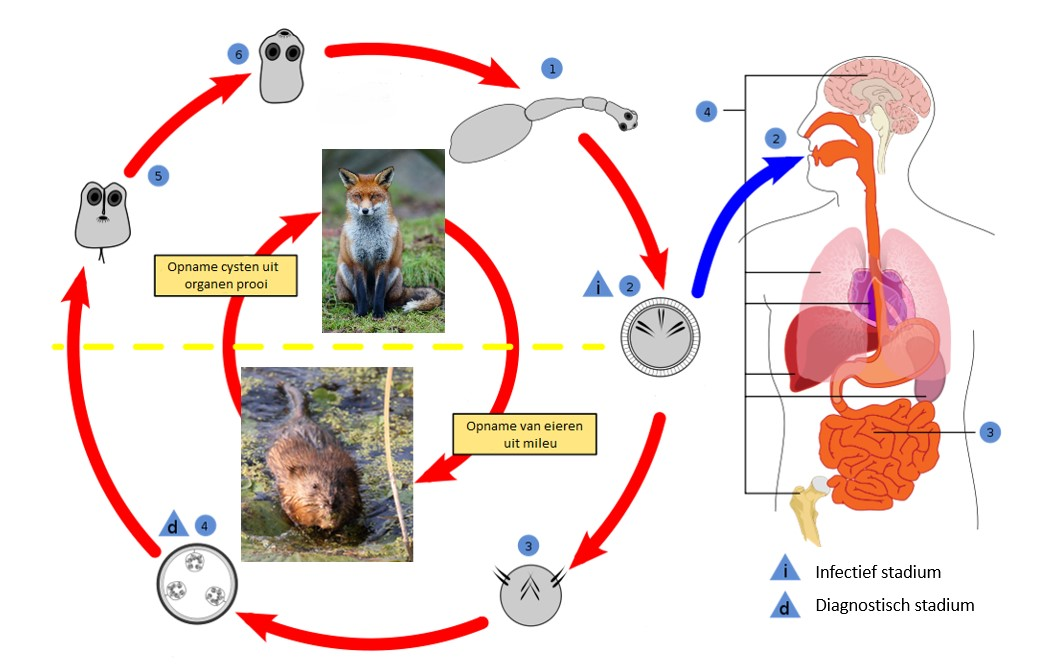
\includegraphics[width=1\linewidth]{col} 

}

\caption{Levenscyclus EM: Buitenste cirkel: 1. Volwassen
lintworm in dunne darm 2. Eieren in uitwerpselen 3. Oncosfeer boort door
de darmwand en komt in bloedbaan terecht 4. Metacestode in lever 5.
Protoscoleces in darmstelsel eindgastheer 6. Vasthechting aan darmwand,
Binnenste cirkel: gastheer waarin de respectievelijke EM stadia van de
buitenste cirkel zich bevinden, de gele stippelijn duid de overgang
tussen tussengastheer en eindgastheer aan (© D. Richfield 2014).}\label{fig:Levenscyclus}
\end{figure}

\subsection{Vrijlevend ei-stadium}\label{vrijlevend-ei-stadium}

De rijpe EM eieren komen via de uitwerpselen van de eindgastheer in de
buitenwereld. Ze hebben een diameter van 30 tot 40µm diameter en
bevatten het eerste larve-stadium (de oncosfeer) van de lintworm. De
oncosfeer wordt gekenmerkt door 6 bewegelijke haken en is omgeven door
een eikapsel bestaande uit verschillende lagen. Eén van die lagen is de
resistente, sterk gekeratiniseerde embryophore. De EM eieren zijn
morfologisch niet te onderscheiden van die van lintwormen van het genus
\emph{Taenia} \citep{eckert2001oie}. Eens ze de eindgastheer hebben
verlaten zijn de eieren onderhevig aan verschillende omgevingsfactoren.
EM eieren kunnen doorheen het jaar geruime tijd infectieus blijven
\citep{veit1995influence}. Uit laboratoriumtesten bleek bovendien dat de
eieren 240 dagen temperaturen tot -18°C kunnen weerstaan maar binnen de
twee dagen sterven bij -83°C. Ook bij te hoge temperaturen sterven de
eieren snel af. \citet{federer2015vivo} tonen aan dat de eieren
temperaturen tot 65°C kunnen overleven zolang de blootstelling beperkt
is in tijd (niet meer dan 3 uur) en er voldoende luchtvochtigheid is. In
een drogere omgeving blijkt de overleving (infectiviteit) van de eieren
sterk af te nemen. Deze gevoeligheden worden ook teruggevonden op
ruimtelijk grotere schaal. \citet{staubach2001geographic} vonden meer
geïnfecteerde vossen in open landschappen met een vochtige bodem, en
lagere percentages in droger bosgebied.

\subsection{Ontwikkeling in de
tussengastheer}\label{ontwikkeling-in-de-tussengastheer}

Verschillende kleine zoogdieren kunnen als tussengastheer voor EM
optreden, waaronder ook bevers (\emph{Castor fiber}), hazen (\emph{Lepus
europaeus}) en beverratten (\emph{Myocastor coypus})
\citep{romig2017ecology}. Het zijn echter de woelrat (\emph{Arvicola
amphibius}), de veldmuis (\emph{Microtus arvalis}) en de muskusrat die
als de belangrijkste tussengastheren in Europa worden beschouwd
\citep{eckert2001oie}. Ze behoren alle drie tot de onderfamilie van de
woelmuizen of Arvicolinae. Recent onderzoek van
\citet{oksanen2016geographical} geeft ons een indicatie van de
prevalentie van EM in deze soorten in België en buurlanden (Tabel
\ref{tab:prevtussengastheer}). De prevalentie van 16\% in muskusratten
in België is berekend op basis van twee studies uit Wallonië
\citep{mathy2009carriage, hanosset2008echinococcus}. Belangrijk (ten
opzichte van Vlaanderen) hierbij is dat de regio ten noorden van de
Samber-Maas-lijn slechts een prevalentie van 2,02\% (95 \% CI:
1,08--3,43\%) vertoont.

\begin{longtable}[]{@{}llllll@{}}
\caption{\label{tab:prevtussengastheer} Percentage met EM besmette
muskusratten en andere Arvicolinae in België en buurlanden
\citep{oksanen2016geographical}. () = 95\% Confidence interval, * =
gebaseerd op slechts één studie.}\tabularnewline
\toprule
& België & Nederland & Duitsland & Luxemburg & Frankrijk\tabularnewline
\midrule
\endfirsthead
\toprule
& België & Nederland & Duitsland & Luxemburg & Frankrijk\tabularnewline
\midrule
\endhead
Muskusrat & 16,0 (7,0 - 28,0) & 0,06* & 3,8 (2,8 - 4,9) & 1,8* & 1,1
(0,2 - 2,8)\tabularnewline
Arvicolinae & 0,2 (0,0 - 0,6) & & 0,6 (0,4 - 1,0) & & 4,8 (1,6 -
9,7)\tabularnewline
\bottomrule
\end{longtable}

De prevalentie die we zien bij de tussengastheer weerspiegelt deze van
de eindgastheer. In geval van screening bij de tussengastheer dient dit
wel grondiger te gebeuren aangezien de gemiddelde prevalentie van alle
tussengastheren ongeveer één derde van de prevalentie bij de
eindgastheer bedraagt \citep{oksanen2016geographical}.

Eenmaal een lintwormei opgenomen is door een tussengastheer, komt onder
de opeenvolgende invloed van de enzymen in de maag en de darm de
oncosfeer vrij uit het eikapsel. De oncosfeer bestaat slechts uit een
beperkt aantal, sterk gespecialiseerde cellen en wordt het eerste
larvestadium genoemd. Gal aanwezig in de dunne darm activeert de
oncosfeer en door middel van de beweeglijke haken en bepaalde secreties
dringt ze door de darmwand. Eens in de submucosa wordt de oncosfeer
passief via de bloedsomloop getransporteerd naar de lever of meer
uitzonderlijk naar longen, hersenen of andere organen
\citep{eckert2001oie}.

\newpage

Hier begint de oncosfeer aan de metamorfose naar het tweede
larvestadium, de metacestode. De oncosfeer bevat een klein aantal
ongedifferentieerde stamcellen die aan de basis liggen van deze
metamorfose, terwijl de meeste gedifferentieerde cellen verloren gaan
tijdens de transitie. Op dit punt is de parasiet het meest gevoelig voor
de immunologische respons van de tussengastheer. De metacestode bestaat
uit een verzameling vesikels (cel-organellen). Deze vesikels
vermeerderen zich en kunnen zich in het lichaam verspreiden en dwars
door aangrenzend weefsel groeien en zodoende ernstige aandoeningen
veroorzaken. Binnen deze vesikels ontstaan broedkapsels waarin de
protoscoleces zich ontwikkelen. Grote hoeveelheden protoscoleces worden
binnen de 40 tot 60 dagen na infectie al aangemaakt. Het zijn deze
protoscoleces die zich in de eindgastheer elk tot een individuele
lintworm zullen ontwikkelen. De sterke ontwikkeling van de metacestode
kan ertoe leiden dat de tussengastheer minder mobiel wordt en dus een
makkelijke prooi vormt voor een predator, een mogelijke eindgastheer
\citep{eckert2001oie}.

De eieren kunnen ook opgenomen worden door zoogdieren die losstaan van
de levenscyclus. Men spreekt dan van een aberrante of toevallige
gastheer. Dit kan onder meer het geval zijn bij de mens maar ook bij
o.a. everzwijnen (\emph{Sus scrofa}), honden (\emph{Canis lupus
familiaris}), hazen (\emph{Lepus europaeus}) en varkens (\emph{Sus
scrofa domesticus})
\citep{oksanen2016geographical, chaignat2015brown, romig2017ecology}.

\subsection{Ontwikkeling in de
eindgastheer}\label{ontwikkeling-in-de-eindgastheer}

De vos (\emph{Vulpes vulpes}) is de belangrijkste eindgastheer van
\emph{Echinococcus multilocularis} in Europa. In bepaalde streken kunnen
andere carnivoren zoals de wasbeerhond (\emph{Nyctereutes
procyonoides}), de wilde kat (\emph{Felis silvestris}) of de wolf
(\emph{Canis lupus}) als eindgastheer optreden. Ook huiskatten
(\emph{Felis catus}) of honden kunnen deze parasiet dragen. In België is
hier nog geen onderzoek naar verricht, maar wel in Frankrijk, Luxemburg,
Duitsland en Nederland. In Frankrijk werd een prevalentie van 1.5\% bij
huiskatten en 0.4\% bij honden gevonden, in Duitsland was dit
respectievelijk 0.6 en 0.3\%, in Nederland 0.3\% bij huiskatten en geen
geïnfecteerde honden en in Luxemburg werden geen geïnfecteerde
huiskatten of honden gevonden \citep{oksanen2016geographical}.

In onze buurlanden vinden we dus een erg lage prevalentie bij huiskatten
en honden. \citet{hegglin2013control} berekenden echter dat, zelfs bij
een geringe prevalentie van 0.3 tot 0.4\%, honden 10\% kans hebben om
ooit in hun leven geïnfecteerd te raken. Aangezien honden in veel hogere
aantallen in urbane omgevingen voorkomen dan vossen kunnen zij
substantieel bijdragen aan de hoeveelheid lintwormeieren in de directe
nabijheid van mensen. Zo zouden 4-15\% van de eieren in rurale en 7-19\%
van de eieren in urbane gebieden afkomstig zijn van honden.
Geïnfecteerde katten daarentegen scheiden slechts kleine hoeveelheden
eieren uit, \citet{kapel2006reproductive} vonden bovendien dat deze niet
infectieus zijn.

De eindgastheer raakt besmet met de parasiet door het eten van
geïnfecteerde prooien. De protoscoleces afkomstig uit de organen van de
tussengastheer ontwikkelen zich in de dunne darm tot (adulte) lintwormen
en voeden zich met de darminhoud van de eindgastheer. De volwassen
lintworm is slechts enkele millimeter groot en bestaat gemiddeld uit
vijf proglotiden of segmenten \citep{eckert2004biological}. Na een
prepatente periode van 26 tot 29 dagen worden tot 100.000 eieren per dag
geproduceerd \citep{kapel2006reproductive}. Deze excretie kan tot vier
maanden duren \citep{eckert2001oie}. Eens de eieren uitgescheiden zijn
in het milieu kan de cyclus opnieuw van voor af aan beginnen.

\newpage

\section{Verspreiding}\label{verspreiding}

Zuid-Duitsland, Zwitserland, alpien Oostenrijk en bepaalde zones in
Rusland (rond Moskou, Kazan en Tomsk) worden historisch als endemisch
besmet gebied beschouwd \citep{eckert2017historical}. De Europese
besmette regio vertoont sinds de jaren 1970 een uitbreiding naar het
noorden, westen en oosten. Zo observeerden \citet{combes2012westward}
een sterke westwaartse uitbreiding van de vossenlintworm in vossen in
Frankrijk. In Nederlands Limburg werd dan weer een noordwaartse
verspreiding gevonden en werd berekend dat deze verspreiding zich
voordoet met een snelheid van 2,7 km per jaar
\citep{takumi2008evidence}.

\citet{vervaeke2006spatial} zien ook een noordwestwaartse uitbreiding
van de infectie in vossen in België, beginnende vanuit het zuidoosten
van het land. Zij observeren echter ook dat in 2000-2002 de verspreiding
ter hoogte van de gewestgrens lijkt te stabiliseren. Dit zien we ook
terugkomen in de recent opgemaakte kaart van de verspreiding binnen
Europa (Fig. \ref{fig:preval}), waar Wallonië een prevalentie kent
tussen 5 en 25\%, en de prevalentie in Vlaanderen tussen de 0 en 1\%
bedraagt \citep{eckert2017historical}.






\begin{figure}

{\centering 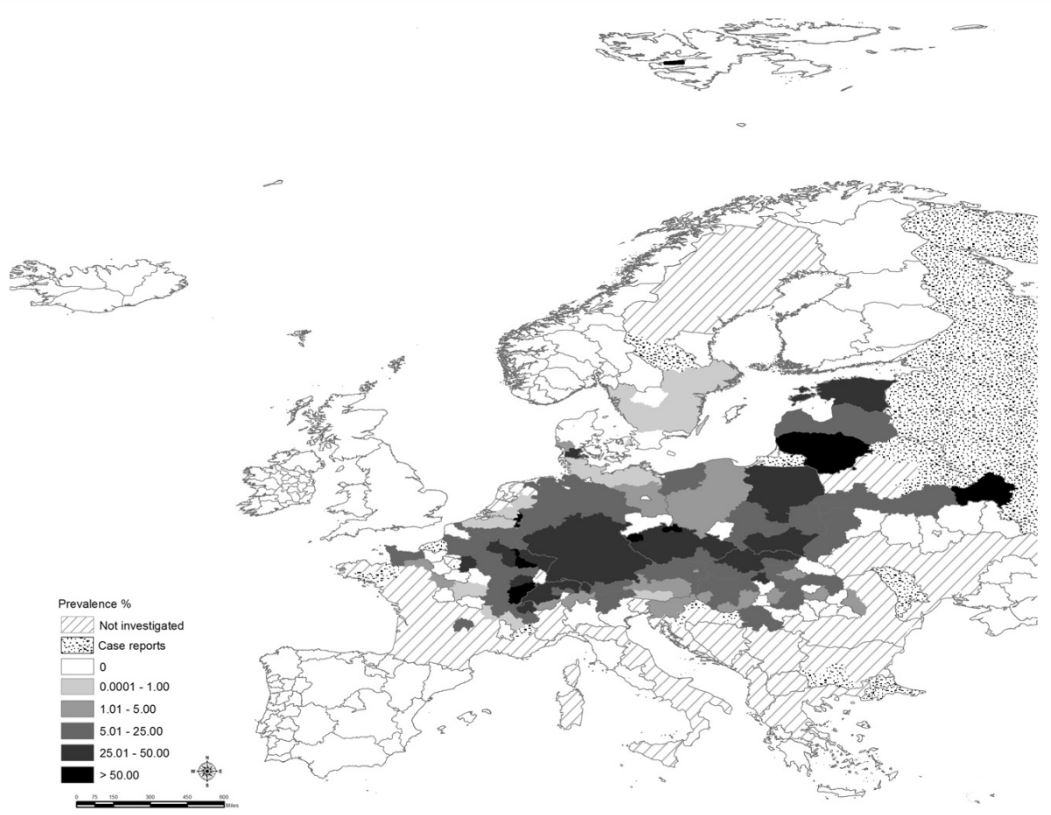
\includegraphics[width=1\linewidth]{Distribution} 

}

\caption{Huidige prevalentie van EM in de eindgastheer in Europa. In
de gestippelde gebieden is geen data over prevalentie in de eindgastheer
beschikbaar maar er zijn wel gevallen bekend van EM infectie van
tussengastheren of de mens (naar \citet{deplazes2017global}).}\label{fig:preval}
\end{figure}

\newpage

\begin{longtable}[]{@{}lllllll@{}}
\caption{\label{tab:prevvossen} Prevalentie van EM in vossen en muskusratten
in België.}\tabularnewline
\toprule
\begin{minipage}[b]{0.20\columnwidth}\raggedright\strut
Locatie\strut
\end{minipage} & \begin{minipage}[b]{0.13\columnwidth}\raggedright\strut
Jaar\strut
\end{minipage} & \begin{minipage}[b]{0.06\columnwidth}\raggedright\strut
Vossen\strut
\end{minipage} & \begin{minipage}[b]{0.07\columnwidth}\raggedright\strut
\% besmet\strut
\end{minipage} & \begin{minipage}[b]{0.09\columnwidth}\raggedright\strut
Muskus-\\
ratten\strut
\end{minipage} & \begin{minipage}[b]{0.07\columnwidth}\raggedright\strut
\% besmet\strut
\end{minipage} & \begin{minipage}[b]{0.19\columnwidth}\raggedright\strut
Bron\strut
\end{minipage}\tabularnewline
\midrule
\endfirsthead
\toprule
\begin{minipage}[b]{0.20\columnwidth}\raggedright\strut
Locatie\strut
\end{minipage} & \begin{minipage}[b]{0.13\columnwidth}\raggedright\strut
Jaar\strut
\end{minipage} & \begin{minipage}[b]{0.06\columnwidth}\raggedright\strut
Vossen\strut
\end{minipage} & \begin{minipage}[b]{0.07\columnwidth}\raggedright\strut
\% besmet\strut
\end{minipage} & \begin{minipage}[b]{0.09\columnwidth}\raggedright\strut
Muskus-\\
ratten\strut
\end{minipage} & \begin{minipage}[b]{0.07\columnwidth}\raggedright\strut
\% besmet\strut
\end{minipage} & \begin{minipage}[b]{0.19\columnwidth}\raggedright\strut
Bron\strut
\end{minipage}\tabularnewline
\midrule
\endhead
\begin{minipage}[t]{0.20\columnwidth}\raggedright\strut
Wallonië\strut
\end{minipage} & \begin{minipage}[t]{0.13\columnwidth}\raggedright\strut
1991-1992\strut
\end{minipage} & \begin{minipage}[t]{0.06\columnwidth}\raggedright\strut
85\strut
\end{minipage} & \begin{minipage}[t]{0.07\columnwidth}\raggedright\strut
15\strut
\end{minipage} & \begin{minipage}[t]{0.09\columnwidth}\raggedright\strut
\strut
\end{minipage} & \begin{minipage}[t]{0.07\columnwidth}\raggedright\strut
\strut
\end{minipage} & \begin{minipage}[t]{0.19\columnwidth}\raggedright\strut
\citet{brochier1992enquete}\strut
\end{minipage}\tabularnewline
\begin{minipage}[t]{0.20\columnwidth}\raggedright\strut
Wallonië\strut
\end{minipage} & \begin{minipage}[t]{0.13\columnwidth}\raggedright\strut
1998-2002\strut
\end{minipage} & \begin{minipage}[t]{0.06\columnwidth}\raggedright\strut
709\strut
\end{minipage} & \begin{minipage}[t]{0.07\columnwidth}\raggedright\strut
20.2\strut
\end{minipage} & \begin{minipage}[t]{0.09\columnwidth}\raggedright\strut
\strut
\end{minipage} & \begin{minipage}[t]{0.07\columnwidth}\raggedright\strut
\strut
\end{minipage} & \begin{minipage}[t]{0.19\columnwidth}\raggedright\strut
\citet{losson2003prevalence}\strut
\end{minipage}\tabularnewline
\begin{minipage}[t]{0.20\columnwidth}\raggedright\strut
Wallonië\strut
\end{minipage} & \begin{minipage}[t]{0.13\columnwidth}\raggedright\strut
2003-2004\strut
\end{minipage} & \begin{minipage}[t]{0.06\columnwidth}\raggedright\strut
178\strut
\end{minipage} & \begin{minipage}[t]{0.07\columnwidth}\raggedright\strut
41.6\strut
\end{minipage} & \begin{minipage}[t]{0.09\columnwidth}\raggedright\strut
\strut
\end{minipage} & \begin{minipage}[t]{0.07\columnwidth}\raggedright\strut
\strut
\end{minipage} & \begin{minipage}[t]{0.19\columnwidth}\raggedright\strut
\citet{Flament2004echino}\strut
\end{minipage}\tabularnewline
\begin{minipage}[t]{0.20\columnwidth}\raggedright\strut
Wallonië\strut
\end{minipage} & \begin{minipage}[t]{0.13\columnwidth}\raggedright\strut
2003-2004\strut
\end{minipage} & \begin{minipage}[t]{0.06\columnwidth}\raggedright\strut
993\strut
\end{minipage} & \begin{minipage}[t]{0.07\columnwidth}\raggedright\strut
24.4\strut
\end{minipage} & \begin{minipage}[t]{0.09\columnwidth}\raggedright\strut
1727\strut
\end{minipage} & \begin{minipage}[t]{0.07\columnwidth}\raggedright\strut
11.8\strut
\end{minipage} & \begin{minipage}[t]{0.19\columnwidth}\raggedright\strut
\citet{hanosset2008echinococcus}\strut
\end{minipage}\tabularnewline
\begin{minipage}[t]{0.20\columnwidth}\raggedright\strut
Wallonië (Ourthe vallei)\strut
\end{minipage} & \begin{minipage}[t]{0.13\columnwidth}\raggedright\strut
2005-2006\strut
\end{minipage} & \begin{minipage}[t]{0.06\columnwidth}\raggedright\strut
\strut
\end{minipage} & \begin{minipage}[t]{0.07\columnwidth}\raggedright\strut
\strut
\end{minipage} & \begin{minipage}[t]{0.09\columnwidth}\raggedright\strut
657\strut
\end{minipage} & \begin{minipage}[t]{0.07\columnwidth}\raggedright\strut
22.1\strut
\end{minipage} & \begin{minipage}[t]{0.19\columnwidth}\raggedright\strut
\citet{mathy2009carriage}\strut
\end{minipage}\tabularnewline
\begin{minipage}[t]{0.20\columnwidth}\raggedright\strut
Brussel\strut
\end{minipage} & \begin{minipage}[t]{0.13\columnwidth}\raggedright\strut
2001-2004\strut
\end{minipage} & \begin{minipage}[t]{0.06\columnwidth}\raggedright\strut
160\strut
\end{minipage} & \begin{minipage}[t]{0.07\columnwidth}\raggedright\strut
0\strut
\end{minipage} & \begin{minipage}[t]{0.09\columnwidth}\raggedright\strut
\strut
\end{minipage} & \begin{minipage}[t]{0.07\columnwidth}\raggedright\strut
\strut
\end{minipage} & \begin{minipage}[t]{0.19\columnwidth}\raggedright\strut
\citet{brochier2007echinococcus}\strut
\end{minipage}\tabularnewline
\begin{minipage}[t]{0.20\columnwidth}\raggedright\strut
Brussel\strut
\end{minipage} & \begin{minipage}[t]{0.13\columnwidth}\raggedright\strut
2007-2008\strut
\end{minipage} & \begin{minipage}[t]{0.06\columnwidth}\raggedright\strut
56\strut
\end{minipage} & \begin{minipage}[t]{0.07\columnwidth}\raggedright\strut
0\strut
\end{minipage} & \begin{minipage}[t]{0.09\columnwidth}\raggedright\strut
\strut
\end{minipage} & \begin{minipage}[t]{0.07\columnwidth}\raggedright\strut
\strut
\end{minipage} & \begin{minipage}[t]{0.19\columnwidth}\raggedright\strut
\citet{van2010no}\strut
\end{minipage}\tabularnewline
\begin{minipage}[t]{0.20\columnwidth}\raggedright\strut
Vlaanderen\strut
\end{minipage} & \begin{minipage}[t]{0.13\columnwidth}\raggedright\strut
1996-1999\strut
\end{minipage} & \begin{minipage}[t]{0.06\columnwidth}\raggedright\strut
237\strut
\end{minipage} & \begin{minipage}[t]{0.07\columnwidth}\raggedright\strut
1.69\strut
\end{minipage} & \begin{minipage}[t]{0.09\columnwidth}\raggedright\strut
\strut
\end{minipage} & \begin{minipage}[t]{0.07\columnwidth}\raggedright\strut
\strut
\end{minipage} & \begin{minipage}[t]{0.19\columnwidth}\raggedright\strut
\citet{vervaeke2003echinococcus}\strut
\end{minipage}\tabularnewline
\begin{minipage}[t]{0.20\columnwidth}\raggedright\strut
Vlaanderen\strut
\end{minipage} & \begin{minipage}[t]{0.13\columnwidth}\raggedright\strut
2007-2008\strut
\end{minipage} & \begin{minipage}[t]{0.06\columnwidth}\raggedright\strut
136\strut
\end{minipage} & \begin{minipage}[t]{0.07\columnwidth}\raggedright\strut
0\strut
\end{minipage} & \begin{minipage}[t]{0.09\columnwidth}\raggedright\strut
\strut
\end{minipage} & \begin{minipage}[t]{0.07\columnwidth}\raggedright\strut
\strut
\end{minipage} & \begin{minipage}[t]{0.19\columnwidth}\raggedright\strut
\citet{van2010no}\strut
\end{minipage}\tabularnewline
\begin{minipage}[t]{0.20\columnwidth}\raggedright\strut
Vlaanderen\strut
\end{minipage} & \begin{minipage}[t]{0.13\columnwidth}\raggedright\strut
10/2012-12/2012\strut
\end{minipage} & \begin{minipage}[t]{0.06\columnwidth}\raggedright\strut
306\strut
\end{minipage} & \begin{minipage}[t]{0.07\columnwidth}\raggedright\strut
1.96\strut
\end{minipage} & \begin{minipage}[t]{0.09\columnwidth}\raggedright\strut
\strut
\end{minipage} & \begin{minipage}[t]{0.07\columnwidth}\raggedright\strut
\strut
\end{minipage} & \begin{minipage}[t]{0.19\columnwidth}\raggedright\strut
\citet{vervaeke2012vossenlintworm}\strut
\end{minipage}\tabularnewline
\begin{minipage}[t]{0.20\columnwidth}\raggedright\strut
Vlaanderen\strut
\end{minipage} & \begin{minipage}[t]{0.13\columnwidth}\raggedright\strut
10/2013-01/2014\strut
\end{minipage} & \begin{minipage}[t]{0.06\columnwidth}\raggedright\strut
303\strut
\end{minipage} & \begin{minipage}[t]{0.07\columnwidth}\raggedright\strut
2.64\strut
\end{minipage} & \begin{minipage}[t]{0.09\columnwidth}\raggedright\strut
\strut
\end{minipage} & \begin{minipage}[t]{0.07\columnwidth}\raggedright\strut
\strut
\end{minipage} & \begin{minipage}[t]{0.19\columnwidth}\raggedright\strut
\citet{vervaeke2014geen}\strut
\end{minipage}\tabularnewline
\begin{minipage}[t]{0.20\columnwidth}\raggedright\strut
Vlaanderen\strut
\end{minipage} & \begin{minipage}[t]{0.13\columnwidth}\raggedright\strut
10/2014-12/2014\strut
\end{minipage} & \begin{minipage}[t]{0.06\columnwidth}\raggedright\strut
316\strut
\end{minipage} & \begin{minipage}[t]{0.07\columnwidth}\raggedright\strut
1.58\strut
\end{minipage} & \begin{minipage}[t]{0.09\columnwidth}\raggedright\strut
\strut
\end{minipage} & \begin{minipage}[t]{0.07\columnwidth}\raggedright\strut
\strut
\end{minipage} & \begin{minipage}[t]{0.19\columnwidth}\raggedright\strut
\citet{vervaeke2014bis}\strut
\end{minipage}\tabularnewline
\bottomrule
\end{longtable}

Uit tabel \ref{tab:prevvossen} blijkt duidelijk dat de prevalentie in
Wallonië een stuk hoger is dan in Vlaanderen. Ook zien we dat de
prevalentie in vossen in Vlaanderen vrij stabiel blijft. Wanneer we
kijken naar de verspreiding (Fig. \ref{fig:vossen}) zien we dat de
meeste geïnfecteerde vossen in Vlaanderen dicht bij de gewestgrens
gevonden worden.




\begin{figure}

{\centering \includegraphics{Vossenlintworm-rapport_files/figure-latex/vossen-1} 

}

\caption{Verspreiding en infectiestatus van onderzochte vossen in
België \emph{(Icon made by Freepik from www.flaticon.com.)}}\label{fig:vossen}
\end{figure}

\section{Risisco voor de mens: Alveolaire echinococcose
(AE)}\label{risisco-voor-de-mens-alveolaire-echinococcose-ae}

\BeginKnitrBlock{exampleblock}{}
Echinococcose is een zoönose (een ziekte overgedragen van dieren op
mensen) veroorzaakt door een besmetting met lintwormen van het genus
\emph{Echinococcus}. Echinococcose bestaat in vier vormen, elk
veroorzaakt door een andere soort lintworm:

\begin{longtable}[]{@{}ll@{}}
\toprule
Ziekte & Soort\tabularnewline
\midrule
\endhead
Cystische echinococcose of hydatidose & \emph{Echinococcus
granulosis}\tabularnewline
Aveolaire echinococcose & \emph{Echinococcus
multilocularis}\tabularnewline
Polycystische echinococcose & \emph{Echinococcus vogeli}\tabularnewline
Unicystische echinococcose & \emph{Echinococcus
oligarthrus}\tabularnewline
\bottomrule
\end{longtable}

De eerste twee vormen, cystische en alveolaire echinococcose, zijn
belangrijk voor de wereldvolksgezondheid. De muskusrat speelt enkel een
rol in de verspreiding van \emph{Echinococcus multilocularis} en het
risico op Alveolaire echinococcose (AE). Tussengastheren voor
\emph{Echinococcus granulosis} zijn hoefdieren, voornamelijk schapen en
geiten, eindgastheren zijn voornamelijk honden maar wilde carnivoren
kunnen deze rol ook opnemen.
\EndKnitrBlock{exampleblock}

\subsection{Infectie, detectie en
behandeling}\label{infectie-detectie-en-behandeling}

De meeste gevallen van AE vinden we in Europa in de leeftijdsgroep
tussen de 50 en 70 jaar, hoewel gevallen vanaf 10 en tot 89 jaar bekend
zijn. De kans is even groot voor mannen als vrouwen om besmet te
geraken. Mensen die actief zijn in de bosbouw, tuinbouw, landbouw,
jagerij, of die een hond of kat (hoewel andere resultaten dit
tegenspreken voor katten, zie hierboven) bezitten hebben een hogere kans
op infectie
\citep{eckert2001oie, vuitton2015clinical, craig2017echinococcosis}.
Belangrijk om op te merken is dat zelfs in endemische gebieden de
prevalentie zeer laag is bij mensen (11-40 gevallen per 100.000
inwoners). De meeste gevallen vinden we bij oudere of immunodeficiëntie
mensen waardoor we kunnen besluiten dat de mens een sterke aangeboren
resistentie tegen AE heeft \citep{eckert2001oie}.

Nadat de eieren via het spijsverteringstelsel opgenomen zijn, ontwikkelt
de oncosfeer zich in de lever tot metacestode op vergelijkbare manier
als bij andere tussengastheren. Dit letsel in de lever is tussen een
paar millimeter en 20 cm groot, soms met centrale necrose tot gevolg.
Van hieruit kan de infectie zich via het lymfe- of bloedvatensysteem
verspreiden naar andere organen. Tussen infectie en het optreden van
symptomen zit bij mensen een incubatietijd van vijf tot vijftien jaar.
De eerste symptomen zijn geelzucht (1/3 van de gevallen) en buikpijn
(1/3 van de gevallen). De overige gevallen worden ontdekt bij onderzoek
naar aanleiding van vermoeidheid, gewichtsverlies, hepatomegalie (een
vergrote lever) of abnormale resultaten van specifieke laboratorium- of
echografie-testen \citep{eckert2001oie}.

Bij een vermoeden van AE op basis van voornoemde symptomen wordt een
echografie of CT-scan uitgevoerd waarbij wordt nagegaan of de lever
vergroot is en de kenmerkende laesies vertoont. Ook biochemisch kan de
parasiet aangetoond worden: bepaalde testen kunnen antilichamen tegen EM
vinden (1/2 van de patiënten vertoont deze), na biopsie van de lever kan
histologisch onderzoek of PCR-analyse uitsluitsel geven
\citep{eckert2001oie}.

De behandeling van AE bestaat uit het chirurgisch verwijderen van de
aangetaste delen van de lever en andere organen. Dit wordt dan gevolgd
door minstens twee jaar chemotherapie. Indien de infectie te
wijdverbreid is en er niet meer geopereerd kan worden, dient levenslang
chemotherapie gevolgd te worden \citep{eckert2001oie}. Wanneer men
tijdig kan ingrijpen, is aangetoond dat Europese patiënten een
vergelijkbare levensverwachting hebben als de rest van de bevolking
\citep{torgerson2008alveolar, piarroux2011clinical}.

\subsection{Prevalentie}\label{prevalentie}

Wereldwijd komen naar schatting een 18.000 gevallen van AE per jaar
voor. Van deze gevallen komt er 91\% voor in China en slechts 8.8\% in
Europa, Rusland en Centraal-Azië. In Noord-Amerika komen dus zeer weinig
gevallen van AE voor. Voor zover gekend beperkt de verspreiding zich tot
het noordelijke halfrond \citep{torgerson2010global}.

De meeste klinische patiënten in Europa worden geregistreerd in het
endemisch gebied gelegen in Zwitserland, Zuid-Duitsland en delen van
Oostenrijk en Frankrijk. In deze gebieden neemt het aantal gevallen van
AE toe en bovendien komen er ook steeds meer gevallen voor waar er
historisch geen voorkwamen, vooral in centraal-oost Europa en de
Baltische landen. Deze toename kan mogelijk verklaard worden door een
toegenomen aandacht voor de ziekte en een betere screening. Maar ook na
het algemeen beschikbaar worden van echografie in de jaren 1970 zet deze
stijgende trend zich verder. Verklaringen voor deze verdere toename
dienen dus eerder gezocht te worden in de toename van het aantal
tussengastheren, en/of de toegenomen vossenpopulatie en hun urbanisatie
\citep{vuitton2015clinical}. Mogelijke andere verklaringen zijn de
toegenomen populariteit van outdoor-activiteiten waardoor mensen meer en
meer het leefgebied van mogelijk besmette dieren betreden. Verder zal de
bevolkingsgroei ook leiden tot hogere absolute aantallen besmette
mensen.

Hoewel België geen historisch endemisch gebied is, zijn ook hier
gevallen van AE bekend. Tussen 1996 en 2000 werden in kader van het
EurEchinoReg project drie gevallen van AE in België gevonden
\citep{kern2003european}. De meest recente gegevens (Fig.
\ref{fig:gevallen}) zijn afkomstig van Sciensano, dat samengesteld is
uit het voormalige Centrum voor Onderzoek in Diergeneeskunde en
Agrochemie (CODA) en het vroegere Wetenschappelijk Instituut
Volksgezondheid (WIV). Zij rapporteren de resultaten van het
referentielaboratorium aan de ULB, waar jaarlijks ongeveer 250 tot 300
serologische testen uitgevoerd worden om antilichaampjes tegen EM te
detecteren \citep{rebodello2017zoonosen}. Bovendien is dit laboratorium
het verzamelpunt waar AE gevallen uit België gemeld kunnen worden,
hoewel dit geen verplichting is in België (Carlier Y., persoonlijke
mededeling).





\begin{figure}

{\centering 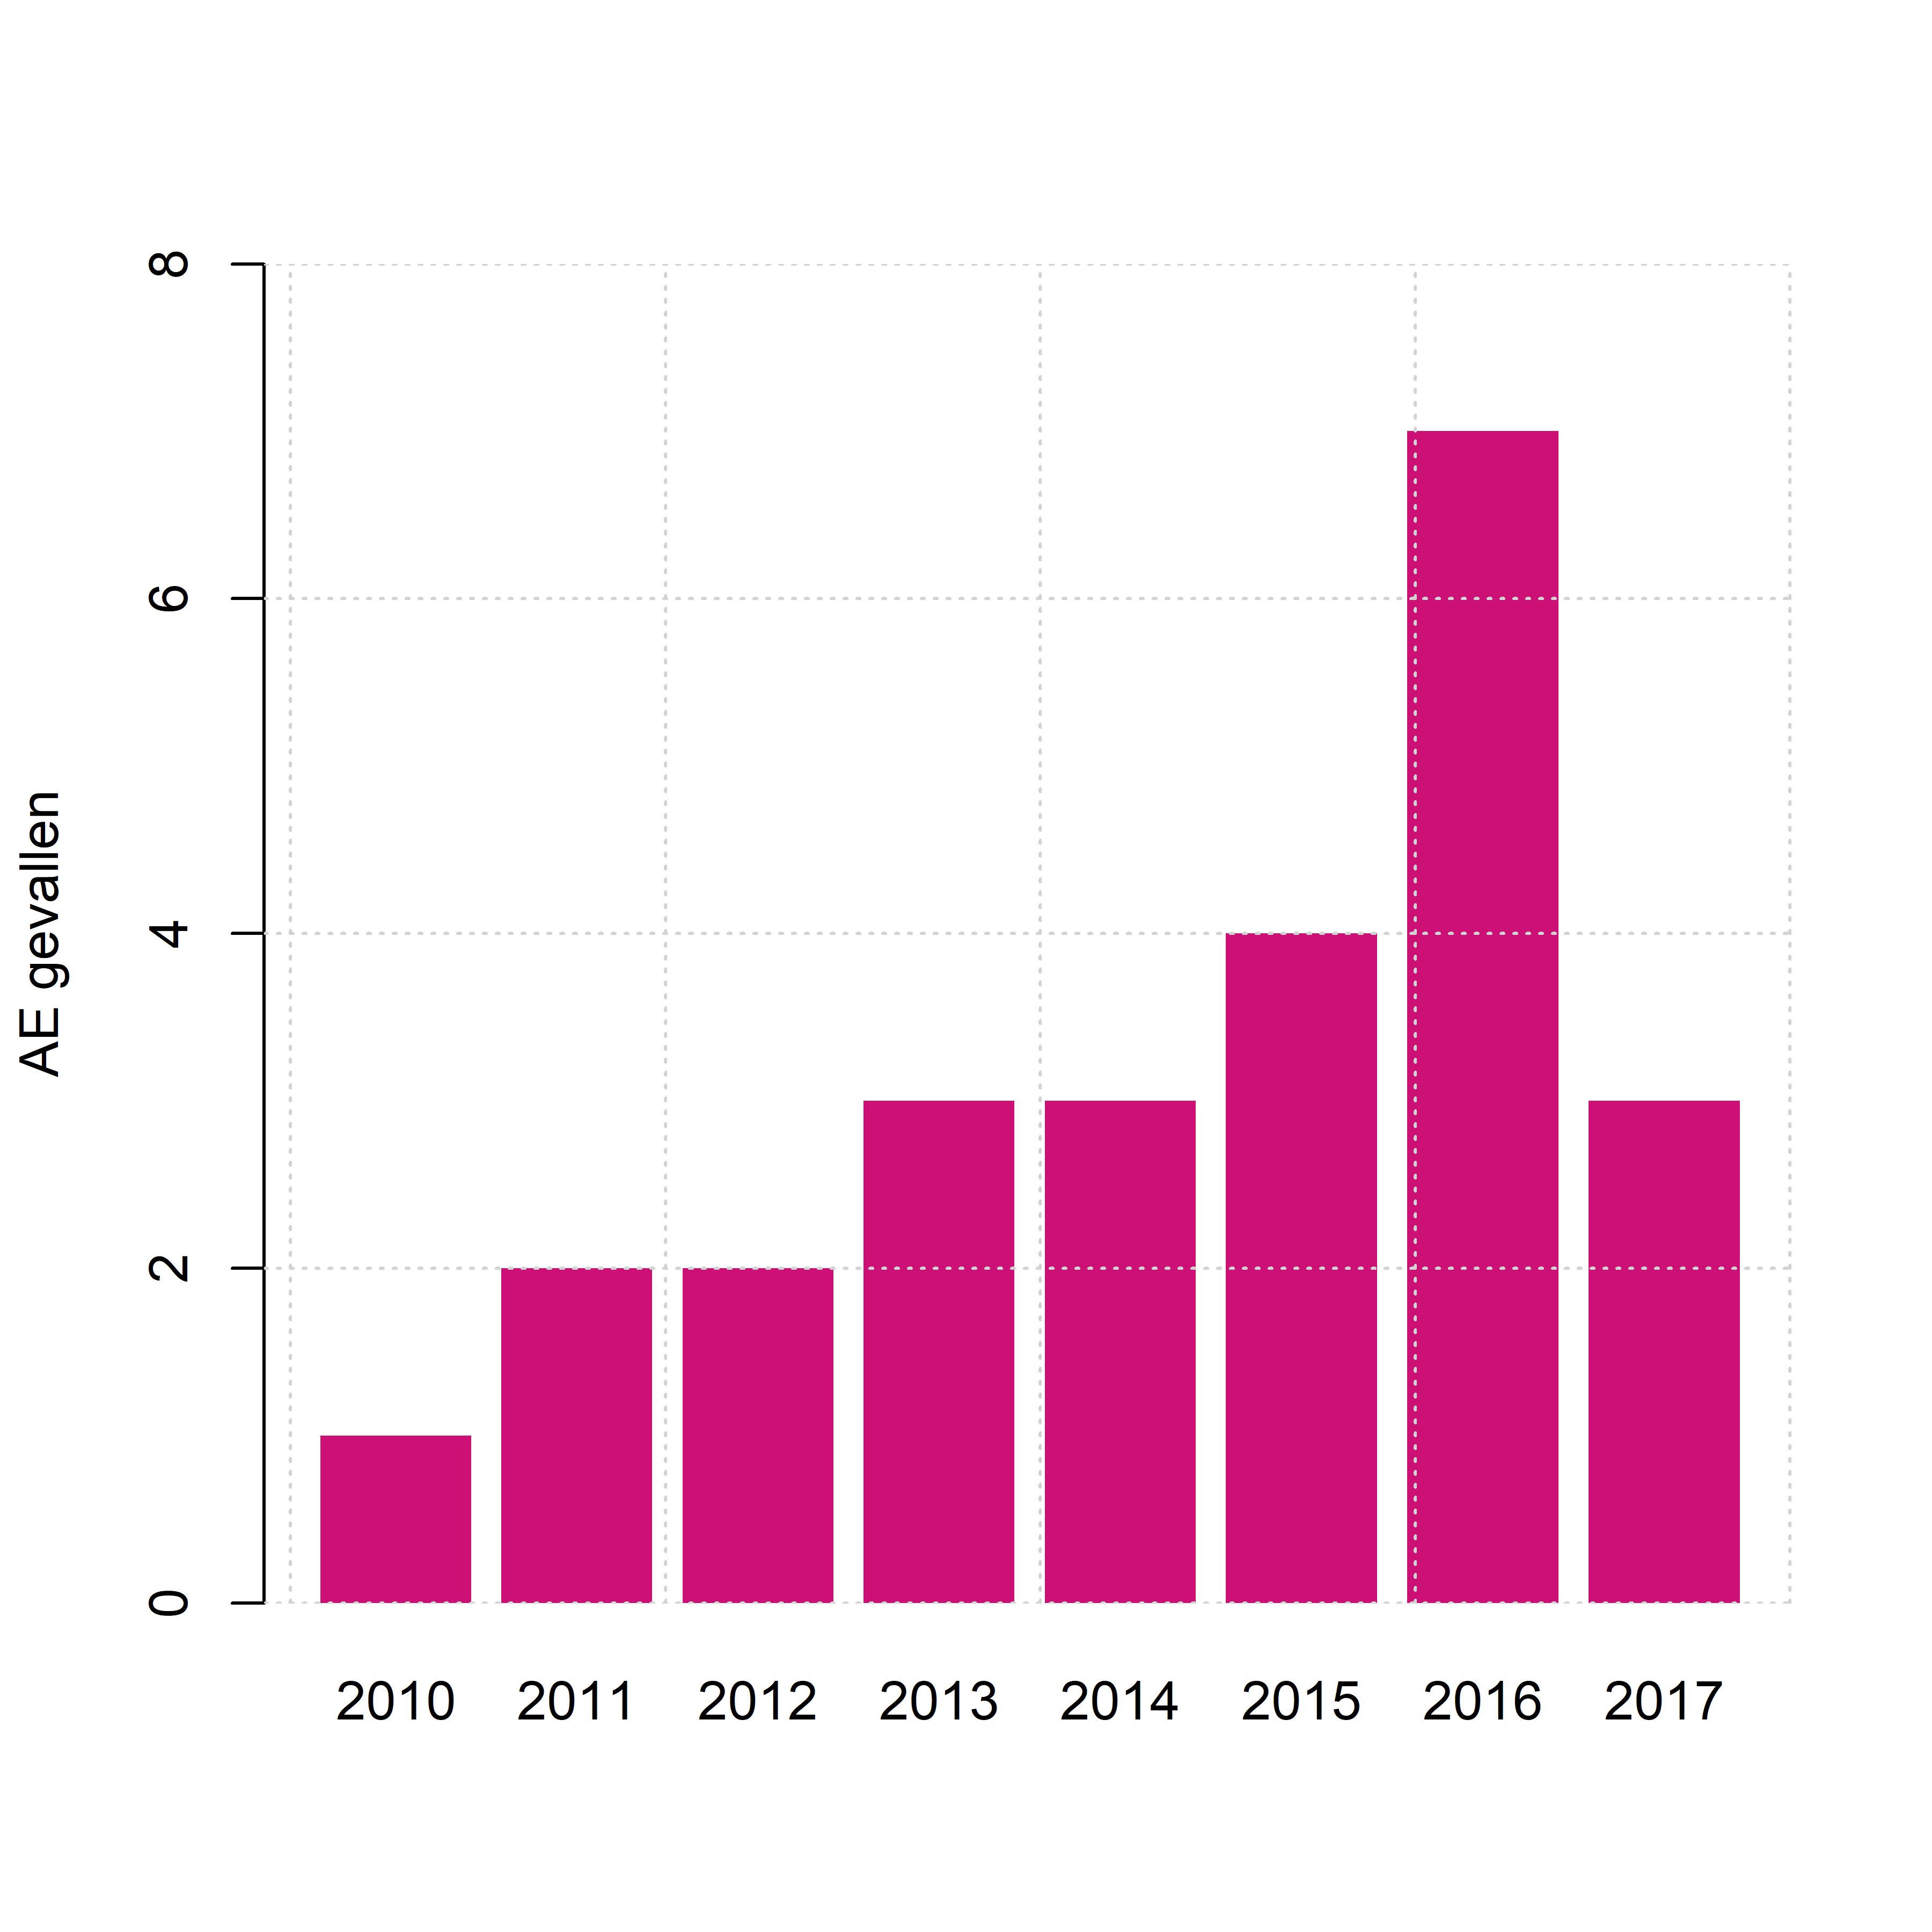
\includegraphics{Vossenlintworm-rapport_files/figure-latex/gevallen-1} 

}

\caption{Aantal gerapporteerde gevallen van alveolaire
echinococcose per jaar in België in de periode 2010-2017
\citep{litzroth2017echinococcus}.}\label{fig:gevallen}
\end{figure}

\chapter{Methodes}\label{methodes}

\section{Sampling van de
muskusratten-populatie}\label{sampling-van-de-muskusratten-populatie}

De muskusratten werden gevangen door de rattenvangers van de VMM in het
kader van de reguliere bestrijding en werden ter beschikking gesteld van
het INBO. De meeste dieren werden een variabele tijd ingevroren bij ca.
-20°C in afwachting van verdere verwerking.

De gegevens (datum en plaats) werden door de rattenvangers genoteerd op
een plastic label dat aan een achterpoot van het gevangen dier werd
vastgemaakt. Bij grotere vangsten werden de dieren niet individueel
gelabeld, maar werden de gegevens op de verpakking genoteerd.

Bij de verwerking op het INBO kregen alle ingezamelde dieren na
ontdooiing een individueel identificatienummer, waaraan alle gegevens
van de verschillende stappen in de verwerking werden gelinkt.

De datum die werd genoteerd, is de datum van de controle van het
vangmateriaal, niet noodzakelijk de de datum waarop de muskutrat in de
val terecht kwam. De vallen worden minimaal elke week gecontroleerd, bij
hoge densiteiten van muskusratten worden vallen meestal dagelijks
gecontroleerd.

De vangstplaats werd afgeleid uit de verschillende locatieaanduidingen
die door de rattenvangers werden genoteerd. Dit kon zijn:

\begin{itemize}
\tightlist
\item
  een gemeente of deelgemeente, een gehucht of een toponiem (domein,
  reservaat, hoeve, \ldots{})
\item
  een beschrijving van de plaats t.o.v. vaste referentiepunten,
  verkeerswegen, spoorwegen, brug \ldots{}
\item
  een waterloop, plas, kreek, \ldots{}
\item
  een hydrografische zone
\item
  Lambert-coördinaten van een plaats, een segment van een waterloop, een
  km²-blok, \ldots{}
\item
  UTM-coördinaten van een plaats of de aanduiding van een UTM km²-hok.
\end{itemize}

Deze aanduidingen of een combinatie ervan werden aanvankelijk in een
databank opgenomen zoals opgegeven door de rattenvanger. In een latere
fase werd getracht de aanduidingen te harmoniseren.

De rattenvangers noteerden zelf ook gegevens betreffende hun
werkzaamheden. Deze werden aanvankelijk genoteerd op vangstformulieren.
Sinds 2016 werd overgestapt op elektronische registratie via smartphone
waarbij ook de vangstlocatie via GPS wordt geregistreerd.

Met behulp van ArcGis en GoogleMaps werd getracht om van elk dier aan de
hand van de aanduidingen op de labels en de beschikbare VMM-data de
vangstplaats zo nauwkeurig mogelijk vast te stellen. Voor de vangsten
van vóór 2016 werd getracht om steeds minstens de gemeente en de
hydrografische zone te achterhalen. Waterlopen vormen echter zeer
frequent tevens een (gemeente)grens, wat de registratie bemoeilijkt.
Voor de periode 2016-2017 werd getracht om op basis van de
label-informatie elke vangst te koppelen aan een elektronische
veldregistratie uit de VMM-databank.

\newpage

\section{Dissecties en visuele controle van de
lever}\label{dissecties-en-visuele-controle-van-de-lever}

Bij het dissecteren van de muskusratten werden
standaard-voorzorgsmaatregelen toegepast. De protoscoleces en/of
germinatieve cellen van de metacestode werden vooraf onschadelijk
gemaakt door de muskusratten in te vriezen. In het laboratorium werden
de ontdooide muskusratten indien nodig ontdaan van vuil (slijk,
bladeren, steentjes, \ldots{}) en overtollig water in de pels. Daarna
werd het gewicht, het geslacht en eventuele verwondingen of
bijzonderheden genoteerd.

Na het opensnijden werd de buikholte nagekeken op mogelijke aanwezigheid
van macroparasieten, waarbij het volledige oppervlak van de lever
geïnspecteerd werd op oneffenheden, verkleuringen, letsels e.d. De
aanwezigheid van cysten in de lever werd als volgt beoordeeld :

\begin{itemize}
\tightlist
\item
  Voor de aanwezigheid van \emph{Taenia taeniaeformis} gebruikten we een
  score van 0 tot 3, in stappen van 0.5, volgens het aantal cysten en de
  impact op het leverweefsel.
\item
  De aanwezigheid dan wel afwezigheid van \emph{Taenia martis} of
  \emph{Taenia crassiceps} in de buikholte werd genoteerd.
\item
  EM aanwezigheid werd gescoord als positief, negatief of onduidelijk.
\item
  Wanneer cysten van EM werden vastgesteld, werden hiervan enkele foto's
  genomen waarop de aard van de infectie duidelijk was. Ook eventuele
  uitzaaiingen werden in beeld gebracht.
\item
  Hoewel in de meeste gevallen de aanwezigheid van EM duidelijk
  herkenbaar is, werd ter bevestiging een preparaatje gemaakt en
  onmiddellijk onder de lichtmicroscoop onderzocht op aanwezigheid van
  hakenkransen (scoleces).
\end{itemize}

\section{Analyse}\label{analyse}

De ruwe dataset bevatte 33699 observaties waarvan er 1278 (4\%)
verwijderd werden wegens het ontbreken van een locatie. De data werden
geanalyseerd met behulp van R (R Core Team, 2018). Data werden
gegroepeerd per parameter en significantie van geobserveerde verschillen
werd getest m.b.v. een Chi-Square test.

\chapter{Resultaten}\label{resultaten}

In de periode van 1994 tot 2017 werden in totaal 32.076 muskusratten
gedissecteerd en onderzocht op het INBO. Bij de dissectie van 1994 tot
2007 van 16.128 muskusratten troffen we geen dieren aan die besmet waren
met vossenlintworm. In 2008 registreerden we een eerste positief dier.
Vanaf 2009 werden daarom alle muskusratten, die door VMM-bestrijders
werden gevangen, ingezameld en aan het INBO onderzocht. In de periode
2009 - 2017 werden 15.402 muskusratten gedissecteerd en gescoord voor
EM. Er werden in diezelfde periode 17.497 muskusratten gevangen door de
VMM. Van alle in deze periode gevangen exemplaren ontbreken er dus 12\%.
Vermoedelijk gaat het over dieren die in te verre staat van ontbinding
waren of de gedissecteerde dieren waaraan geen locatie toegekend kon
worden. De ontbrekende ratten zijn min of meer verspreid over
Vlaanderen, met een piek aan de gewestgrens (Fig. \ref{fig:vmmvang}).
Dit is niet verwonderlijk gezien daar, in absolute aantallen, ook de
meeste muskusratten gevangen worden. Wanneer we kijken naar het totaal
aantal gevangen exemplaren in Vlaanderen, d.w.z. zowel door de VMM als
de provinciale en gemeentelijke rattenvangers gevangen dieren, dan
stellen we wel vast dat een groot deel van de muskusratten uit
West-Vlaanderen niet onderzocht werd (Fig. \ref{fig:allevang}). Dit
omdat enkel de rattenvangers van de VMM en niet de lokale rattenvangers
deelnamen aan dit project.

\begin{figure}

{\centering \includegraphics{Vossenlintworm-rapport_files/figure-latex/vmmvang-1} 

}

\caption{Verschillen tussen door VMM gevangen muskusratten en aantal gedissecteerd muskusratten.}\label{fig:vmmvang}
\end{figure}

\begin{figure}

{\centering \includegraphics{Vossenlintworm-rapport_files/figure-latex/allevang-1} 

}

\caption{Verschillen tussen alle geregisteerde vangsten en aantal gedissecteerd ratten.}\label{fig:allevang}
\end{figure}

\section{Geografische spreiding}\label{geografische-spreiding}

In figuur \ref{fig:kaarten} en \ref{fig:kaarten2} wordt de geografische
verspreiding gegeven van de huidige prevalentiedata in de INBO-databank
betreffende de 32.412 muskusratten die in de loop der jaren werden
gedissecteerd. De gegevens van 1994-2007 worden in één kaartje
samengevat (figuur \ref{fig:kaarten}) gezien er in die periode geen
aanwezigheid van EM werd vastgesteld. Hierbij wordt een idee gegeven van
het aantal en de spreiding van de onderzochte muskusratten. Al de dieren
uit deze periode werden negatief voor EM bevonden.

\begin{figure}

{\centering \includegraphics{Vossenlintworm-rapport_files/figure-latex/kaarten-1} 

}

\caption{Gedissecteerde muskusratten in de periode 1994-2007. Geen van deze muskusratten was besmet met EM.}\label{fig:kaarten}
\end{figure}

De parasiet komt vooral voor in de gewestgrenszone tussen
Spierre-Helkijn en Beersel. Ook duiken enkele positieve gevallen op in
het zuidelijk deel van de provincie Limburg.

\begin{figure}

{\centering \includegraphics{Vossenlintworm-rapport_files/figure-latex/kaarten2-1} 

}

\caption{Percentage geïnfecteerde muskusratten per jaar. Klikken op de gemeente geeft aantal besmette muskusratten/totaal aantal gedissecteerde muskusratten.}\label{fig:kaarten2}
\end{figure}

\section{Opdeling per regio}\label{opdeling-per-regio}

Tabel \ref{tab:regio} geeft het aantal muskusratten dat positief (P)
werd bevonden voor EM en het aantal voor EM negatief (N) bevonden
muskusratten per regio. In een beperkt aantal gevallen kon geen
zekerheid bekomen worden over het al dan niet besmet zijn van het
onderzochte dier (?).

\begin{table}

\caption{\label{tab:regio}Aantal voor EM positief, negatief en onduidelijk bevonden muskusratten per regio.}
\centering
\begin{tabular}[t]{l|r|r|r|r|r|r|r|r|r}
\hline
\multicolumn{1}{c|}{ } & \multicolumn{3}{c|}{Vlaanderen} & \multicolumn{3}{c|}{Wallonië} & \multicolumn{3}{c}{Frankrijk} \\
\cline{2-4} \cline{5-7} \cline{8-10}
jaar & P & N & ? & P & N & ? & P & N & ?\\
\hline
2008 & 0 & 4 & 0 & 1 & 181 & 0 & 0 & 360 & 0\\
\hline
2009 & 3 & 471 & 0 & 50 & 1372 & 8 & 0 & 488 & 0\\
\hline
2010 & 12 & 804 & 1 & 9 & 242 & 1 & 0 & 694 & 0\\
\hline
2011 & 15 & 1190 & 6 & 18 & 299 & 2 & 0 & 664 & 0\\
\hline
2012 & 6 & 887 & 17 & 12 & 331 & 5 & 0 & 389 & 2\\
\hline
2013 & 13 & 664 & 11 & 9 & 140 & 2 & 0 & 136 & 0\\
\hline
2014 & 6 & 1096 & 1 & 13 & 494 & 0 & 0 & 104 & 0\\
\hline
2015 & 8 & 1127 & 0 & 7 & 193 & 0 & 0 & 0 & 0\\
\hline
2016 & 3 & 1249 & 0 & 0 & 112 & 0 & 0 & 0 & 0\\
\hline
2017 & 16 & 1815 & 0 & 2 & 183 & 0 & 0 & 0 & 0\\
\hline
\end{tabular}
\end{table}

De gemiddelde prevalentie bedraagt 3.3\% in Wallonië terwijl deze in
Vlaanderen beperkt blijft tot 0.9\%. Bij de muskusratten uit Frankrijk
werden nog geen besmette dieren aangetroffen. Wanneer we de drie regio's
vergelijken vinden we een significant effect van regio (p \textless{}
0.001). Deze gegevens dienen wel met de nodige voorzichtigheid
geïnterpreteerd te worden aangezien het om opportunistische waarnemingen
uit Wallonië en Frankrijk gaat (soms worden muskusratten net over de
grens gevangen om instroom te voorkomen), in tegenstelling tot de
systematische en gebiedsdekkende inspanning in Vlaanderen.

Wanneer we kijken naar de trend in Vlaanderen (Fig. \ref{fig:trend}) dan
zien we dat het percentage geïnfecteerde muskusratten schommelt rond een
gemiddelde van 0.8\%. Het percentage besmette exemplaren ligt dus erg
laag in Vlaanderen.

\begin{figure}

{\centering 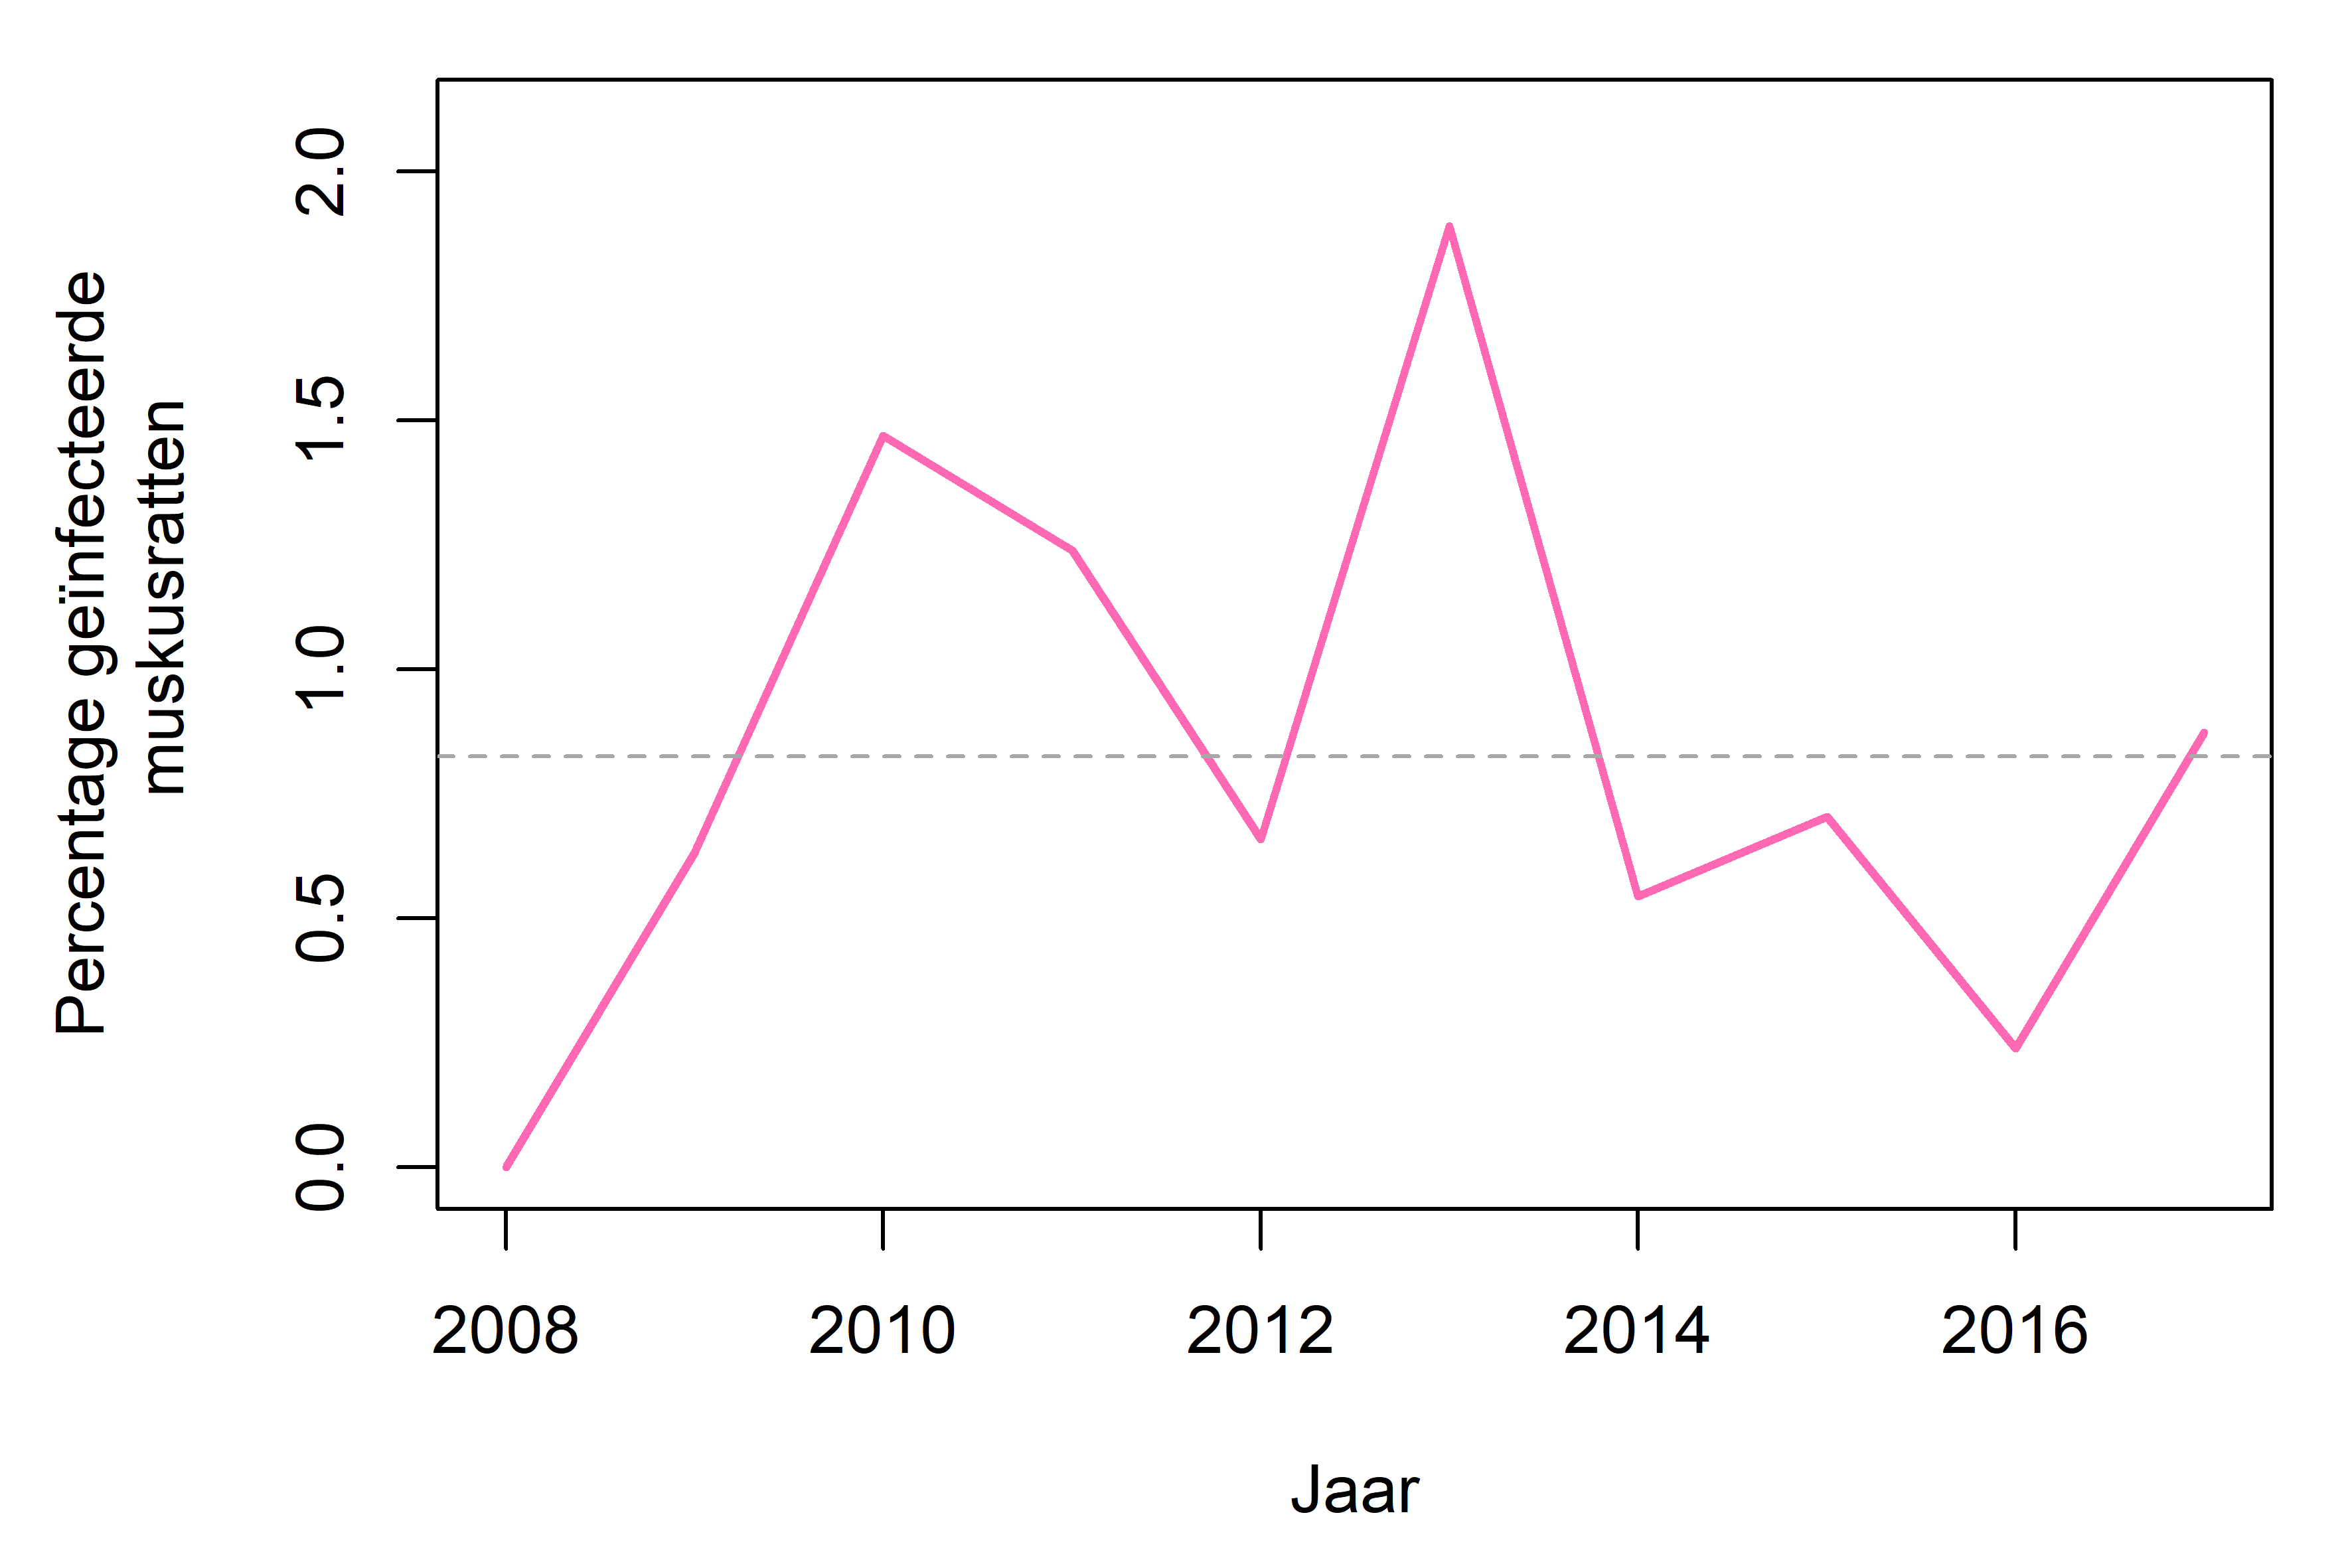
\includegraphics{Vossenlintworm-rapport_files/figure-latex/trend-1} 

}

\caption{Percentage geïnfecteerde muskusratten in Vlaanderen voor de periode 2008 - 2017. De grijze lijn geeft het gemiddelde percentage voor deze periode aan.}\label{fig:trend}
\end{figure}

\section{Opdeling per geslacht}\label{opdeling-per-geslacht}

Er worden meer mannelijke muskusratten gevangen dan vrouwelijke (tabel
\ref{tab:sex}). De sexratio is vergelijkbaar voor alle onderzochte
regio's.

\begin{table}

\caption{\label{tab:sex}Sexratio van alle gevangen muskusratten per regio.}
\centering
\begin{tabular}[t]{l|r|r|r}
\hline
sex & Frankrijk & Vlaanderen & Wallonië\\
\hline
F & 0.44 & 0.42 & 0.43\\
\hline
M & 0.56 & 0.58 & 0.57\\
\hline
\end{tabular}
\end{table}

Wanneer we enkel naar de geïnfecteerde muskusratten kijken zien we dat
ook hier meer mannelijke muskusratten gevangen worden (tabel
\ref{tab:Psex}). In Vlaanderen is het verschil meer uitgesproken dan in
Wallonië, waar we eenzelfde ratio zien als hierboven.

\begin{table}

\caption{\label{tab:Psex}Sexratio van geïnfecteerde muskusratten per regio.}
\centering
\begin{tabular}[t]{l|r|r}
\hline
sex & Vlaanderen & Wallonië\\
\hline
F & 0.35 & 0.42\\
\hline
M & 0.65 & 0.58\\
\hline
\end{tabular}
\end{table}

Er is echter geen significant verschil (p = 0.27) tussen de ratio
man/vrouw bij niet-geïnfecteerde versus geïnfecteerde muskusratten in
Vlaanderen.

\section{Opdeling per
lichaamsgewichtsklasse}\label{opdeling-per-lichaamsgewichtsklasse}

Figuur \ref{fig:dist} toont de distributie van de lichaamsgewichten van
alle gedissecteerde muskusratten gevangen in Vlaanderen. Onder normale
omstandigheden (geen bestrijding) verwachten we dat deze gewichten een
normale verdeling vertonen. De data tonen echter een links-scheve
distributie. Met lichaamsgewicht als proxy voor leeftijd toont dit aan
dat er relatief meer jonge dieren gevangen worden.

\begin{figure}

{\centering 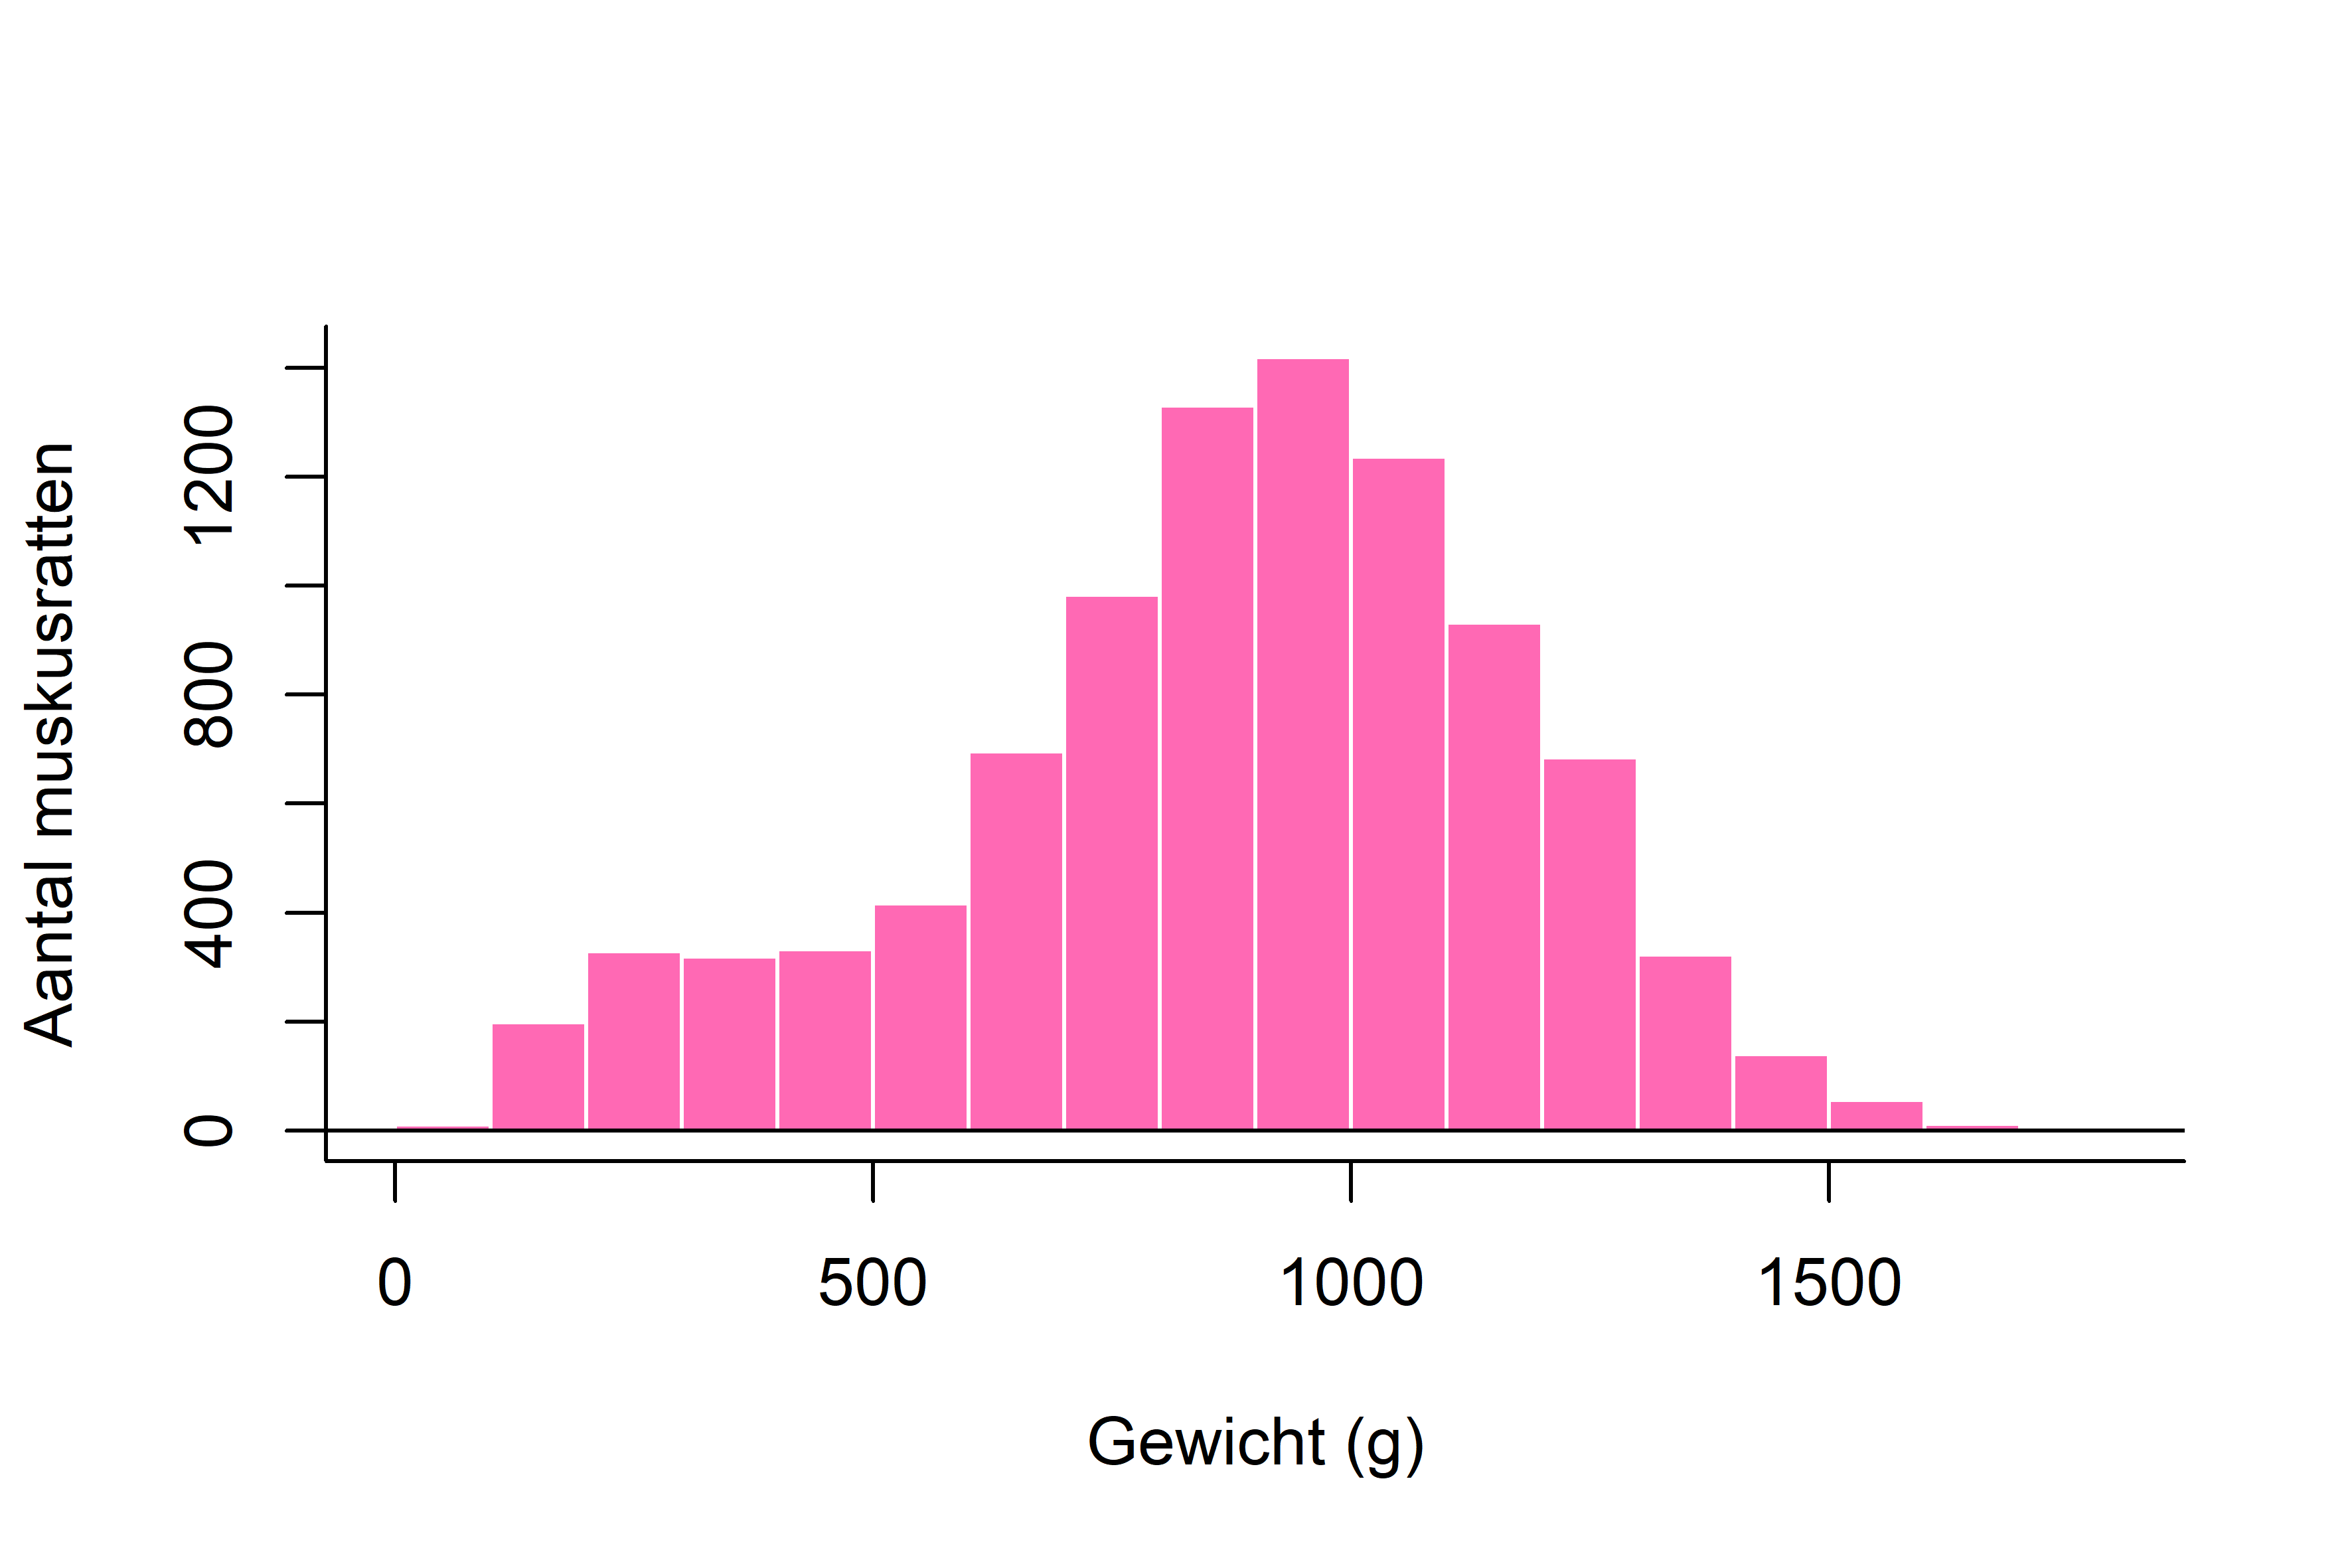
\includegraphics{Vossenlintworm-rapport_files/figure-latex/dist-1} 

}

\caption{Distributie van lichaamsgewichten van alle uit Vlaanderen onderzochte muskusratten.}\label{fig:dist}
\end{figure}

Vanaf het spenen loopt een jonge muskusrat het risico om besmet te
geraken met de lintwormeieren. De kans op besmetting neemt toe naarmate
het dier langer en actiever aanwezig is op het terrein. Na opname van
EM-eieren neemt ook de kans geleidelijk toe dat er cysten in de lever
worden gedetecteerd. Met een toenemende leeftijd mag dan ook een toename
van de kans op een zichtbare infectie verondersteld worden. Wanneer we
het lichaamsgewicht gebruiken als proxy voor de leeftijd, blijkt dit ook
uit onze resultaten (Figuur \ref{fig:geinfgew}). Het feit dat er geen
besmette dieren met een gewicht \textgreater{} 1500g vinden kan
verklaard worden doordat dit een zeer kleine cohorte is (75 dieren).

\begin{figure}

{\centering 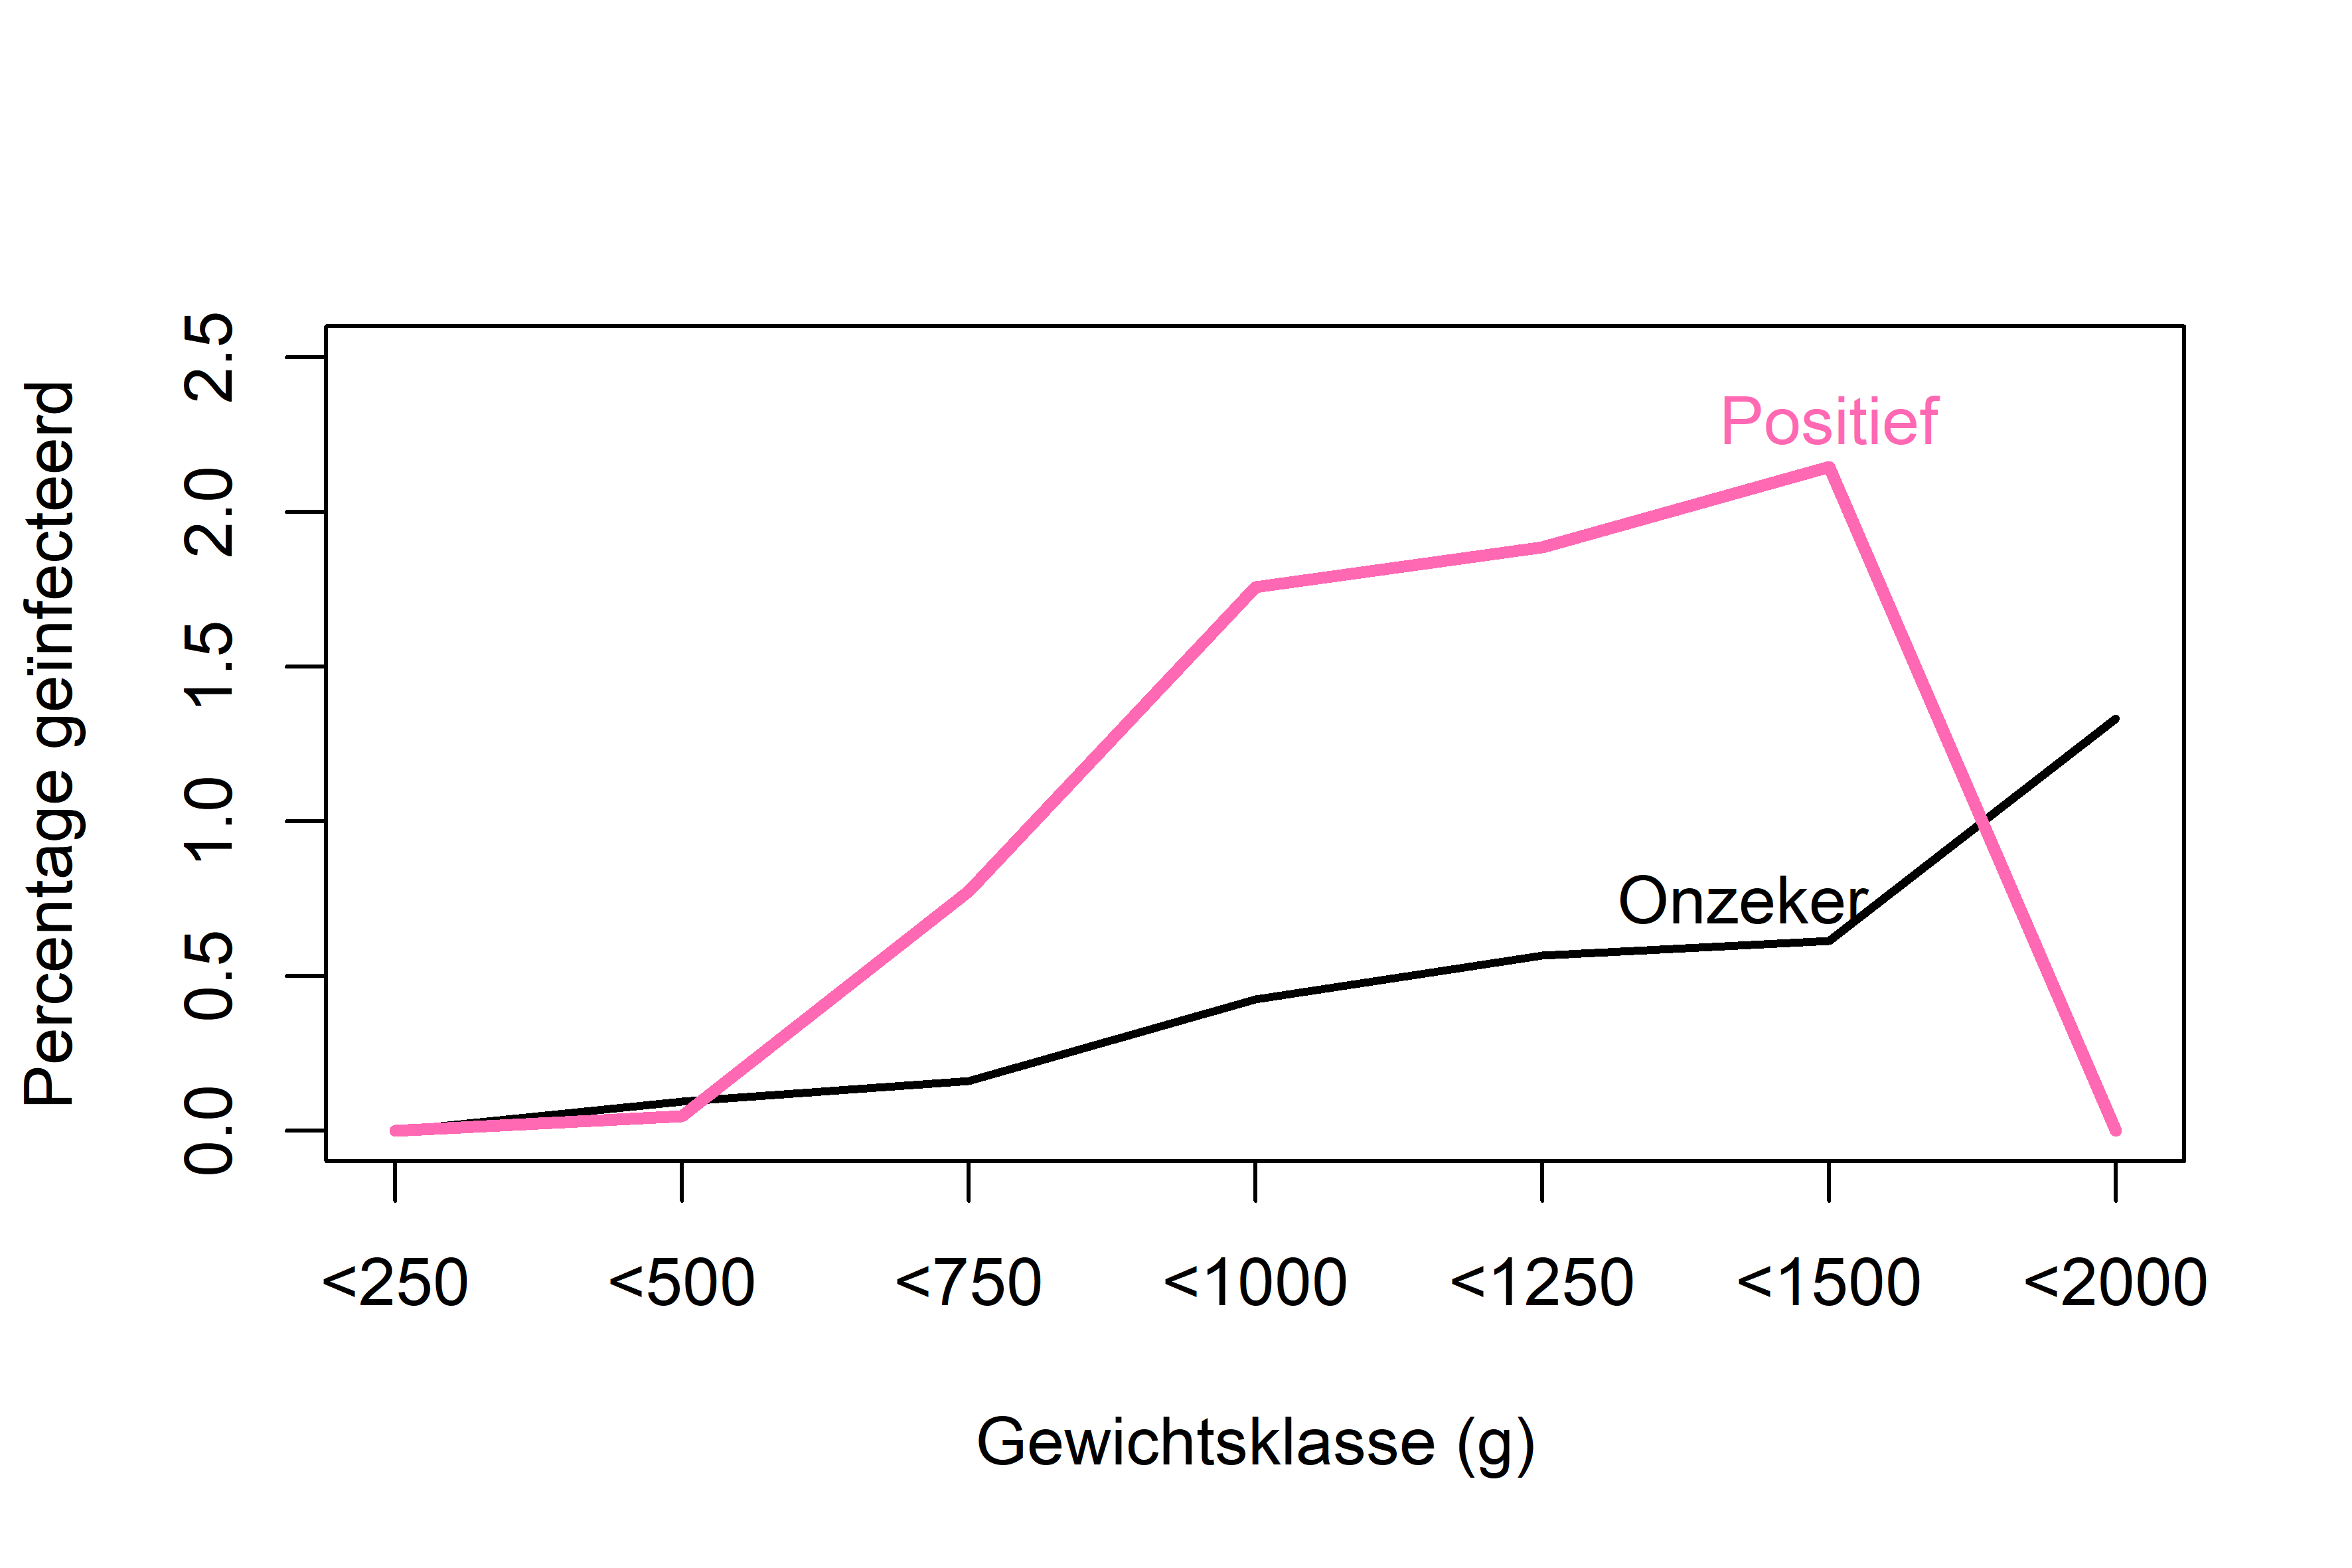
\includegraphics{Vossenlintworm-rapport_files/figure-latex/geinfgew-1} 

}

\caption{Percentage geïnfecteerde (roze) en onzekere (zwart) muskusratten per gewichtsklasse (g).}\label{fig:geinfgew}
\end{figure}

Uit figuur \ref{fig:geinfgew} is af te leiden dat de infectiekans van
muskusratten onder de 500 gram bijzonder laag is in vergelijking met
zwaardere/meer volwassen dieren. We zien ook dat het aantal onduidelijke
gevallen toeneemt met het gewicht. Mogelijk komt dit door een
opstapeling van andere parasieten in de lever, zo blijkt bijvoorbeeld
ook dat er een positieve correlatie is tussen het lichaamsgewicht van de
muskusrat en de graad van infectie met \emph{Taenia taeniaeformis}
(correlatie = 0.49, p \textless{} 0,001).

\section{Opdeling per maand}\label{opdeling-per-maand}

Figuur \ref{fig:geinfmaand} toont de percentages geïnfecteerde en
onzekere dieren ten opzichte van elkaar.

\begin{figure}

{\centering 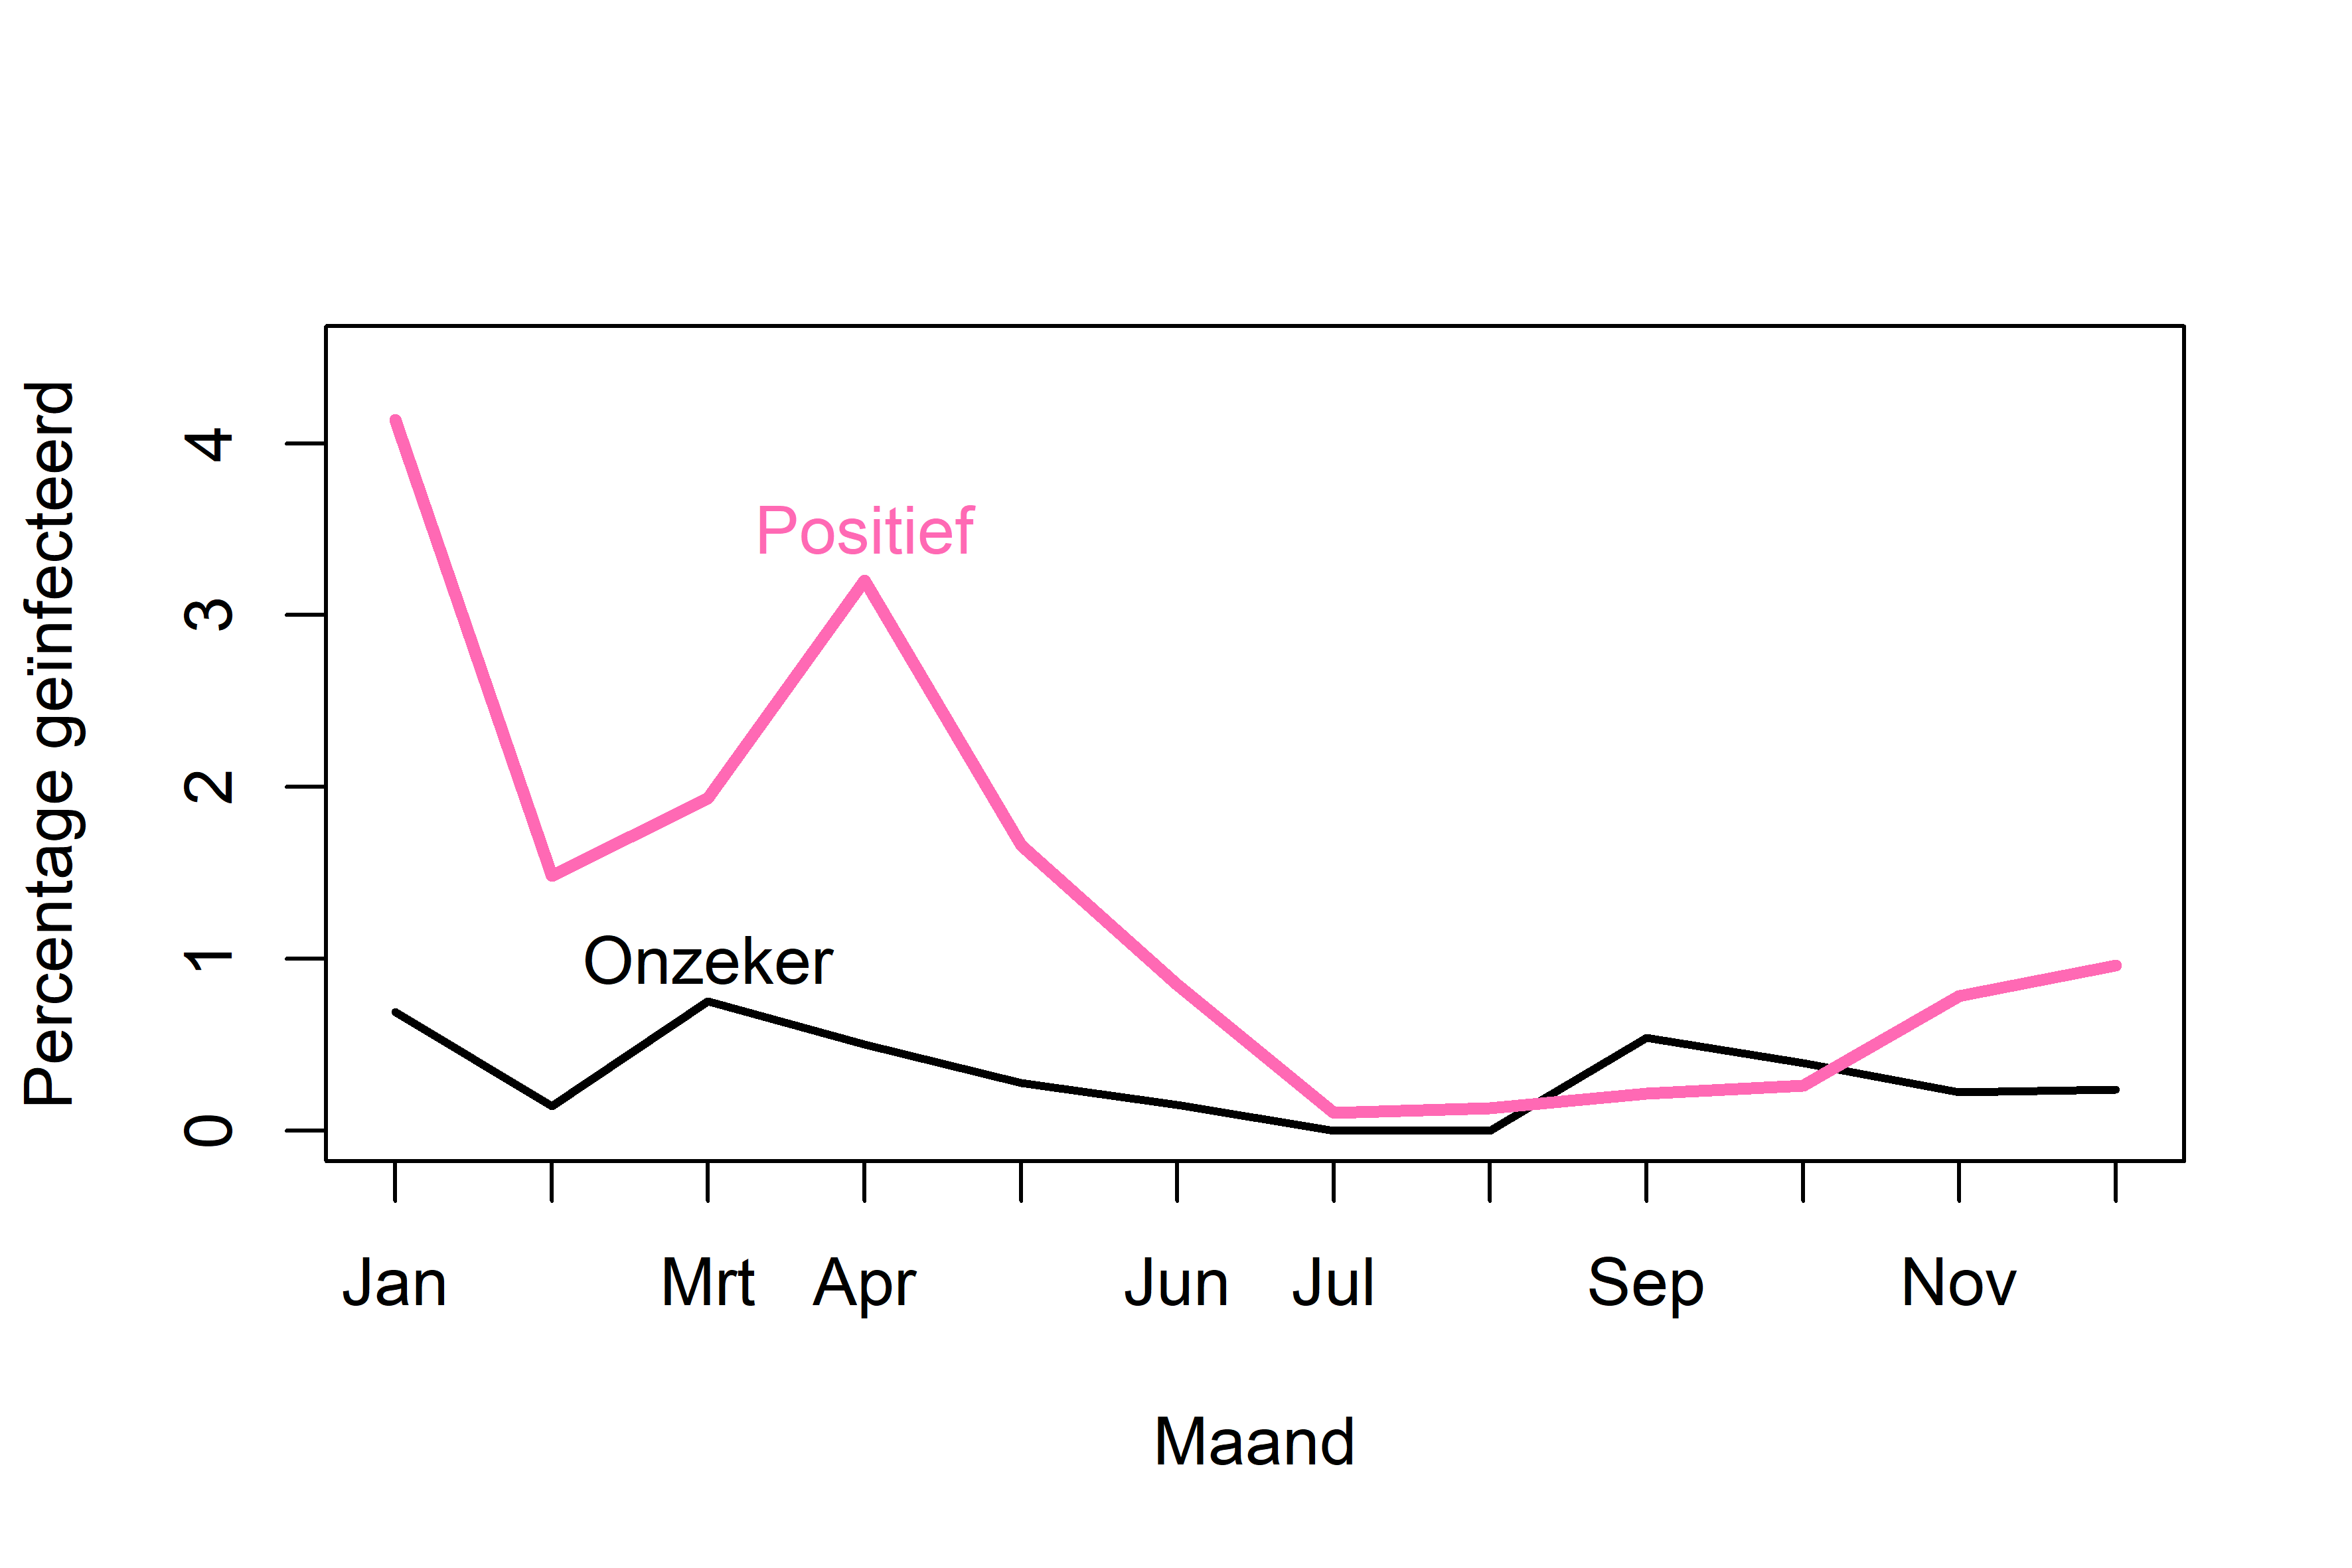
\includegraphics{Vossenlintworm-rapport_files/figure-latex/geinfmaand-1} 

}

\caption{Percentage geïnfecteerde (roze) en onzekere (zwart) muskusratten per maand.}\label{fig:geinfmaand}
\end{figure}

Het grootste percentage besmette muskusratten vinden we in het voorjaar.
Gezien de seizoenale voortplanting van de muskusrat, verandert de
leeftijdsstructuur van de populatie tijdens het jaar. Het percentage
jonge dieren stijgt drastisch vanaf mei terwijl in het najaar minder
jongen geboren worden. De voorjaarspopulatie bestaat overwegend uit
overwinterde subadulte dieren en een kleinere fractie oudere dieren
(\textgreater{} 1 jaar) (Fig. \ref{fig:gewichtsverdeling}). Dit
verklaart dan ook deels het verschil in prevalentie tussen beide
jaarhelften.

\begin{figure}

{\centering 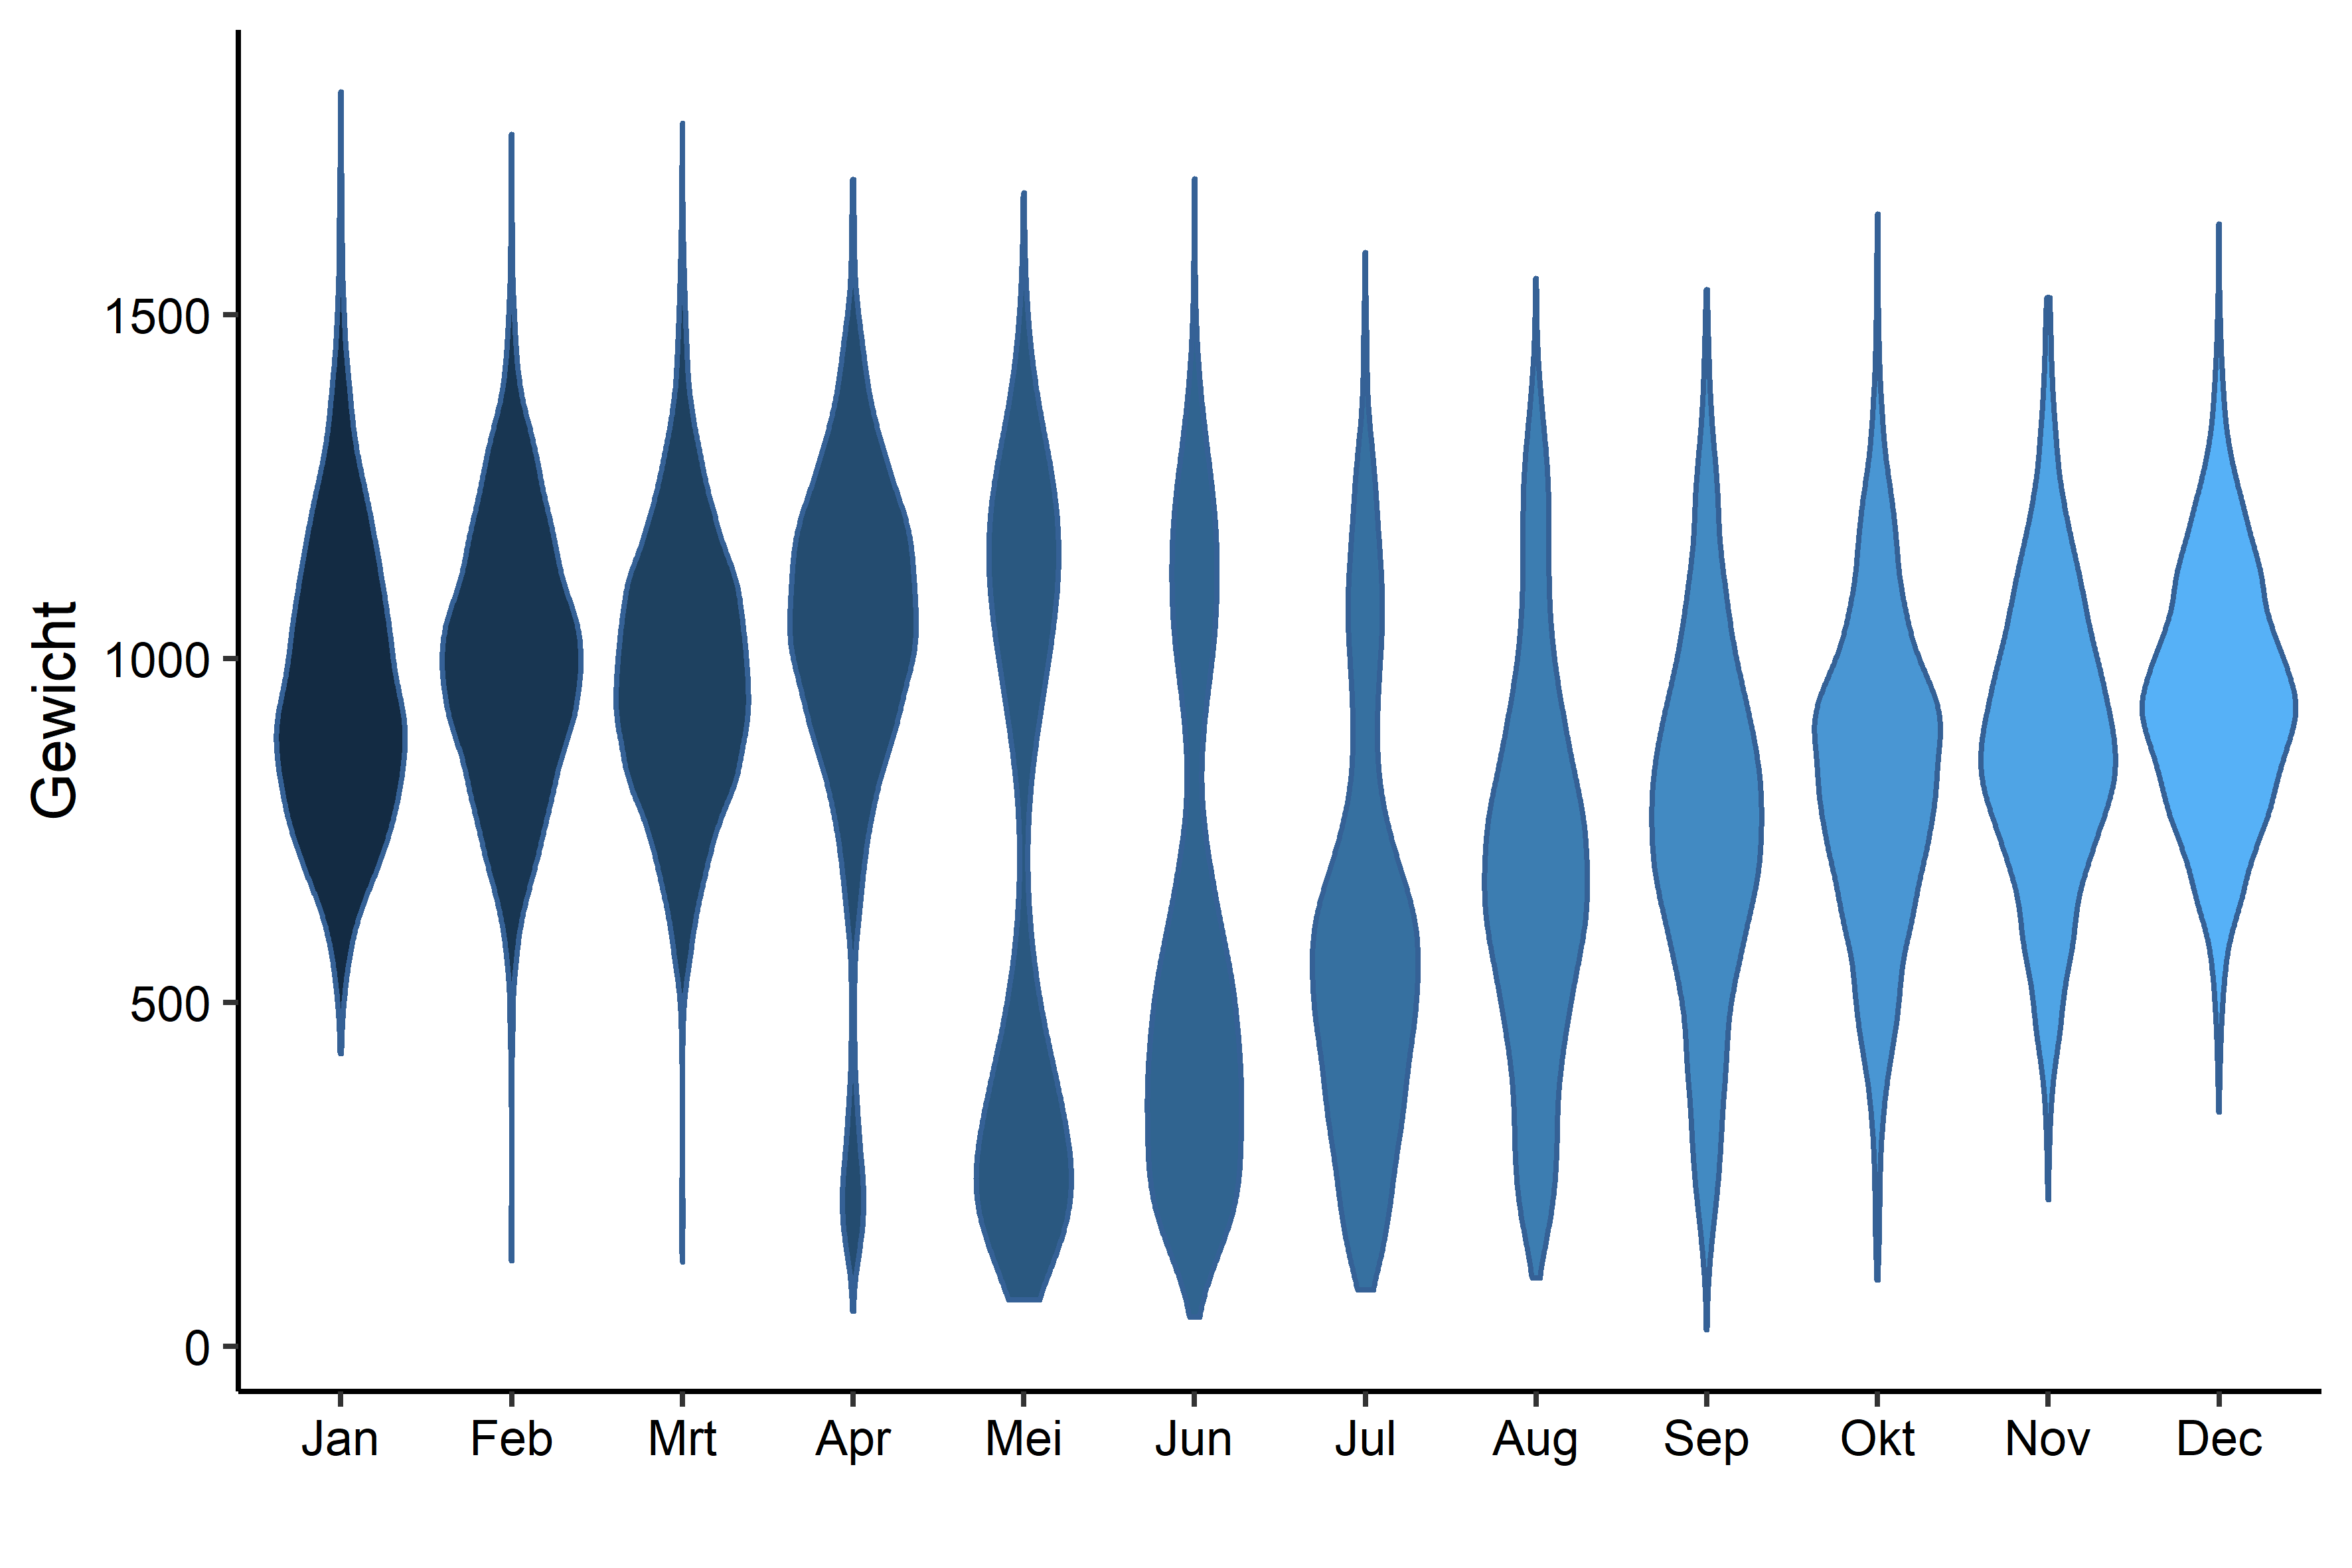
\includegraphics{Vossenlintworm-rapport_files/figure-latex/gewichtsverdeling-1} 

}

\caption{Distributie van het lichaamsgewicht van de gedissecteerde muskusratten per maand.}\label{fig:gewichtsverdeling}
\end{figure}

\chapter{Discussie}\label{discussie}

Het percentage geïnfecteerde muskusratten schommelt rond een gemiddelde
van 0.8\% in Vlaanderen, wat een lage infectiegraad is. Binnen de
periode waarin alle door de VMM gevangen muskusratten onderzocht werden
(2009 -- 2017) merken we bovendien geen stijgende trend. De parasiet
komt vooral voor in de gewestgrenszone tussen Spierre-Helkijn
(West-Vlaanderen) en Beersel (Vlaams-Brabant). Daarnaast duiken enkele
positieve gevallen op in het zuiden van de provincie Limburg. We vinden
de parasiet in Vlaanderen dus enkel in muskusratten gevangen dicht bij
de gewestgrens.

De vraag die we ons moeten stellen is of dit aantoont dat de parasiet
permanent in Vlaanderen aanwezig is, dan wel of het gaat om trekkende
muskusratten die de infectie in Wallonië opgelopen hebben. Muskusratten
trekken vooral in het voorjaar als jong-adulten wanneer ze op zoek gaan
naar een partner, mannetjes trekken hierbij verder dan de vrouwtjes en
worden hierdoor ook vaker gevangen tijdens de trek
\citep{plug1988handboek}. We vinden inderdaad meer mannelijke dieren en
alle dieren gevangen in Vlaanderen vertonen een links-scheve distributie
van de gewichten, wat wijst op een relatief hoog aandeel jonge dieren.
Uit onze data blijkt echter ook dat jongere dieren een lagere kans
hebben besmet te zijn dan oudere dieren, en dat er niet significant meer
mannelijke muskusratten zijn bij de besmette muskusratten. Bovendien is
weinig gekend over de symptomen van en mortaliteit door EM-infectie bij
muskusratten. We weten dus niet hoe waarschijnlijk het is dat een
geïnfecteerd dier over langere afstand gaat migreren. Het blijft dus
onduidelijk of muskusratten de infectie hier in Vlaanderen oplopen of de
besmetting van over de gewestgrens, waar de prevalentie duidelijk hoger
is, meebrengen.

Wanneer we de globale verspreiding van álle onderzochte muskusratten
(niet-geïnfecteerde + geïnfecteerde exemplaren) beschouwen, stellen we
vast dat het overgrote deel van de dieren gevangen wordt aan de
gewestgrens. Aangezien vossenlintworm in vossen en andere
tussengastheren (i.c. diverse kleinere woelmuissoorten) wel nog
verspreid over Vlaanderen voorkomt, is het monitoren van de
vossenlintworm in de muskusrat geen goede proxy om zicht te hebben op
het algemeen voorkomen van de vossenlintworm.

In samenspraak met VMM werd dan ook beslist om niet langer jaarlijks
alle muskusratten in te zamelen en te dissecteren, maar slechts om de
vijf jaar en dan gedurende één jaar. Er werd dus gekozen voor een
spreiding in tijd en niet in plaats. Hoewel we momenteel een goed beeld
hebben waar geïnfecteerde muskusratten voorkomen, is het niet uit te
sluiten dat de infectie ook op andere plaatsen kan opduiken. Om
eventuele lokale infecties bij muskusratten op te sporen zou, rekening
houdend met de (actuele) lage prevalentiegraad, echter een zeer hoge
proportie van de muskusratpopulatie dienen onderzocht te worden. Dit zou
er dan in de praktijk op neerkomen dat zo goed als alle gevangen
exemplaren zouden moeten worden ingezameld. Het inzamelen en het
onderzoeken van gevangen muskusratten afkomstig van Wallonië en
Frankrijk kan in deze vijfjarige cyclus worden verder gezet. Deze
informatie `van over de grens' is immers zeer nuttig om de
vaststellingen bij de muskusratten die in Vlaanderen worden gevangen,
beter te kunnen plaatsen.

\newpage

\section{Mogelijke beheeropties}\label{mogelijke-beheeropties}

\subsection{Sensibilisering, preventie}\label{sensibilisering-preventie}

De bekendste transmissieroute van vossenlintworm naar de mens is via
orale opname van lintwormeitjes \citep{torgerson2008alveolar}. Zoals
hoger geschetst komen de eitjes in het milieu terecht via de
vossenuitwerpselen en kunnen ze in gepaste (o.a. niet-uitdrogende)
omstandigheden weken tot maanden infectieus blijven.

Veelal wordt gewaarschuwd om geen laaggroeiende wilde bessen te eten uit
de natuur. Vaak heerst daarbij het misverstand dat vossen mogelijk
geürineerd zouden kunnen hebben op dergelijke vruchten -- maar de
excretie van eitjes gebeurt niet via de urine. Een (theoretische)
veronderstelling bestaat erin dat vossen op hun pels of aan hun poten
mogelijk eitjes zouden kunnen meedragen, die vervolgens uitgerekend bij
passage doorheen vruchtstruiken toevallig op bessen zouden kunnen
terechtkomen. Deze eitjes op de pels of aan de poten zouden voordien op
het dier terecht moeten gekomen zijn, op plekken die vaak gefrequenteerd
worden en waar regelmatig uitwerpselen liggen, zoals aan burchtsites.
Een andere theoretische veronderstelling slaat op de mogelijkheid dat
kleine partikels van vossenuitwerpselen op de bessen terecht komen, bv.
via insecten of de poten van foeragerende (kleine) vogels en zoogdieren.
Er is echter geen bewijs dat dit een belangrijke rol speelt bij de
besmetting met EM
\citep{kreidl1998domestic, kern2004risk, piarroux2013populations}.

Wel blijkt duidelijk dat personen die regelmatig buitenactiviteiten
verrichten, zoals landbouwers, jagers, tuinders en mensen die veel in
bossen vertoeven, een verhoogd risico lopen. In de praktijk moet een
besmetting zich voordoen via toevallige opname van vossenlintwormeitjes,
bv. door contact tussen mond (lippen) en handen tijdens
buitenwerkzaamheden. Een verhoogde waakzaamheid voor symptomen en
eventueel een regelmatige medische screening bij risicogroepen kunnen
ervoor zorgen dat AE in een vroeg stadium wordt opgespoord en dus beter
behandelbaar is. Dit is echter enkel zinvol in regio's met een hoge
prevalentie. In dergelijke gebieden is het wel belangrijk dat moestuinen
en plaatsen waar laaggroeiend fruit (aardbeien, \ldots{}) geteeld wordt,
goed afgesloten zijn voor honden en vossen zodat daar geen uitwerpselen
(potentiële concentratiehaarden van EM-eitjes) terecht komen, en dat het
voedsel goed gewassen wordt alvorens geconsumeerd te worden
\citep{kreidl1998domestic, kern2004risk, piarroux2013populations}.
Aangezien Vlaanderen een lage prevalentie kent van EM zijn systematische
screeningen naar AE en rigoureus afsluiten van moestuinen e.d. niet in
proportie tot het (zeer geringe) risico op besmetting. Sensibilisatie
rond het goed schoonmaken van groenten en laaggroeiend fruit is wel een
optie, alsook rond het in acht nemen van elementaire
hygiëne-maatregelen, zoals het wassen van de handen voor het eten.

Zoals hoger aangehaald kunnen honden, als mogelijke eindgastheer, een
belangrijke rol spelen in het verspreiden van EM-eieren en kunnen zij
aldus een rechtstreekse bron vormen voor besmetting van mensen. Het is
dan ook zeer belangrijk om honden regelmatig te ontwormen met
ontwormingsmiddelen op basis van praziquantel, zeker als ze mogelijk
tussengastheersoorten van de EM-cyclus (woelmuizen) vangen en effectief
opeten in een gebied met een hoge EM-prevalentie. Ook honden
geïmporteerd vanuit endemische EM-gebieden of honden die tijdelijk in
dergelijke gebieden verbleven (bv. tijdens vakanties), moeten zeker
ontwormd worden. Bovendien moet men er in deze situaties ook een goede
hygiëne op nahouden in het omgaan met honden, o.m. bij wandelingen. Via
hun poten of pels -- zoals na het rollen op de bodem, typisch op sterk
geurende plekken zoals waar uitwerpselen gelegen hebben -- kunnen de
dieren mogelijk EM-eitjes in de directe nabijheid van de mens brengen.

Een specifieke relatie waarbij een hond als mogelijke overbrenger van
EM-eitjes naar de mens toe kan fungeren, wordt gegenereerd door de
zogenaamde `burchtjacht' op vossen
\citep{fauna2009advies, vandenberge2011grote}. Bij een dergelijke
jachtwijze laat men een daartoe getrainde jachthond een vossenburcht
binnendringen, om de vos eruit te drijven zodat die kan geschoten
worden, of om een nest vossenwelpen samen met de moervos te elimineren.
De honden zijn net klein genoeg om in een vossenhol te kunnen kruipen
maar tegelijk voldoende groot om het ondergrondse gevecht met een vos
aan te kunnen. Bij een dergelijke actie schuren de honden dan ook
onvermijdelijk met hun pels veelvuldig tegen de binnenwanden van de
burcht, en komen ze in rechtstreeks intens contact met de vos(sen) zelf
-- waarbij deze tijdens de soms felle ondergrondse gevechten doorgaans
ook defeceren. Gezien burchtsites veelvuldig door vossen worden
gefrequenteerd kunnen zij sowieso als mogelijke hotspots beschouwd
worden voor aanwezigheid van EM-eitjes. Bij intensieve interactie op
zo'n site, wordt de kans zeer reëel dat de mens (de vossenjager, zijn
auto, tuin, \ldots{}) via de jachthond in contact komt met de
lintwormeitjes. Burchtjacht op vos -- als jachtwijze in Vlaanderen niet
toegelaten -- is dan ook als een bijzondere hoog-risicohandeling te
beschouwen ten aanzien van mogelijke besmetting met EM.

Een andere mogelijke route waarbij een permanente en opmerkelijke
nabijheid tussen mens en vos aan de orde komt, is de toename van
stadsvossen \citep{deplazes2004wilderness}. Deze -- onvermijdelijke --
trend heeft zich inmiddels ook in Vlaanderen voltrokken
\citep{vandenberge2013stadsvos}. Toch hoeven urbane vossenpopulaties
niet automatisch tot een hoger risico op EM-besmetting aanleiding te
geven, wegens het mogelijk ontbreken van de nodige
tussengastheerpopulaties in het stedelijk milieu. Overigens leven, zeker
in Vlaanderen, ook rurale vossen nagenoeg overal en onvermijdelijk in
nauw contact met de menselijke bewoning wegens onze specifieke
ruimtelijke ordening gekenmerkt door eindeloze lintbebouwing en
verspreide landelijke bewoning
\citep{vandenberge2011grote, vandenberge2013stadsvos, keune2013science}.

\subsection{Ontwormen van
vossenpopulatie}\label{ontwormen-van-vossenpopulatie}

Het ontwormen van de vossenpopulatie is een mogelijke piste om de
prevalentie van EM in vossenpopulaties omlaag te krijgen. Ze is met
wisselend succes getest in enkele Franse en Japanse steden
\citep{comte2013fox, inoue2007use}. In rurale gebieden blijkt ontworming
er in te slagen de prevalentie van EM te verlagen
\citep{schelling1997chemotherapy, tackmann2001field}. Maar anders dan
bij hondsdolheid (waarvoor vossen met succes gevaccineerd zijn door
middel van een lokaas) volstaat het bij EM niet om éénmalig een vos te
behandelen. Een vos kan namelijk telkens opnieuw geïnfecteerd raken door
het eten van een besmette prooi. De periode tussen opname van het
larvale wormstadium (aanwezig in de tussengastheer) en het vestigen van
de adulte lintworm in het darmstelsel van de eindgastheer bedraagt
ongeveer 30 dagen. Om de cyclus te doorbreken dient de vossenpopulatie
daarom om de maand ontwormd te worden \citep{craig2017echinococcosis}.
Hierbij geldt bovendien dat de metacestodes in de tussengastheer en de
eieren in het milieu meerdere maanden kunnen overleven
\citep{veit1995influence}. \citet{comte2013fox} berekenden bovendien dat
het 114\euro{} zou kosten om één 1km\^{}2 plot éénmaal te behandelen.
Voor een gemeente als Voeren (waar in Vlaanderen de meeste besmette
vossen voorkomen) zou dit neerkomen op ongeveer 69.000\euro{} per jaar.

\subsection{Afschot van vossen en
knaagdierbestrijding}\label{afschot-van-vossen-en-knaagdierbestrijding}

Knaagdieren die drager zijn van het infectieuze larvestadium vormen ook
een reservoir voor de parasiet. Aanwezigheid van de parasiet in de
knaagdierpopulatie brengt dan ook het risico met zich mee voor het
opnieuw sluiten van de cyclus door vos of hond en een mogelijke
voortzetting of uitbreiding van de infectie. Zelfs het verwijderen van
alle vossen uit besmet gebied (voor zover mogelijk) blijkt dan geen
goede beheermaatregel, gezien immigrerende of doortrekkende vossen al
snel opnieuw besmet kunnen geraken. Het op grote schaal en duurzaam
bestrijden van woelmuispopulaties, in situaties waarin de
leefomstandigheden voor die soorten gunstig zijn, blijkt in de praktijk
een zeer moeilijk haalbare doelstelling te zijn
\citep{singleton2010rodent}. Het is overigens de vraag of een dergelijke
actie opportuun zou zijn, gezien woelmuizen het stapelvoedsel vormen van
heel wat predatoren, waaronder beschermde roofvogels.

\citet{vervaeke2006spatial} voorspelden dat de in Wallonië geziene
uitbreiding van vossenlintworm zich noordwaarts in Vlaanderen zou
voortzetten. Dit werd echter niet waargemaakt
\citep[\citet{vervaeke2014geen},
\citet{vervaeke2014bis}]{vervaeke2012vossenlintworm}. Recent genetisch
onderzoek \citep{knapp2009genetic} toont echter aan dat de waargenomen
`verspreiding' eerder te danken is aan een toegenomen aandacht voor de
ziekte en niet zo zeer aan een toegenomen distributie. Dit omdat de
subpopulaties van EM genetisch te sterk verschillend zijn om slechts in
de laatste 50 jaar van elkaar afgesplitst te zijn. Blijft echter de
vraag waarom de infectie historisch ook nooit in Vlaanderen is geraakt.
Een mogelijke verklaring is dat er in Vlaanderen te weinig geschikte
tussengastheren aanwezig zijn om de cyclus te vervolledigen. Hoewel
daarover weinig concreet cijfermateriaal voorhanden is, lijkt de
hypothese gewettigd dat woelmuizen in Vlaanderen relatief weinig
voorkomen. Volgens de Rode Lijst \citep{maes2014iucn} blijken, net zoals
de beide woelratsoorten, ook drie (aardmuis, ondergrondse woelmuis en
veldmuis) van de vier kleine woelmuissoorten in de categorie `bijna in
gevaar' te worden gerangschikt. Enkel voor de rosse woelmuis geldt de
categorisering `momenteel niet in gevaar'. Behalve deze laatste soort,
die o.m. in struwelen en houtkanten leeft, zijn de andere kleine
woelmuissoorten meer aan gevarieerde kruidachtige vegetaties zoals
half-natuurlijke graslanden gebonden. Vermoedelijk ligt de relatieve
zeldzaamheid van dergelijke biotopen, door de intensieve bedrijfsvoering
in de Vlaamse landbouw, aan de basis van het eerder geringe voorkomen
van kleine woelmuissoorten. In Wallonië blijken nagenoeg alle kleine
woelmuissoorten daarentegen nog algemeen voor te komen, en zijn er geen
aanwijzingen voor een achteruitgang \citep{libois2006erosion}. Frappant
in dit verband is dat deze soorten in Vlaanderen niet het stapelvoedsel
van de vos uitmaken zoals in de regel het geval is \citep{lloyd1980red},
maar dat de bruine rat de meest gegeten prooisoort is
\citep{van2010no, keune2013science}. We veronderstellen dat het
succesvol laaghouden van de muskusrattenpopulatie de mogelijke pool van
tussengastheren klein gehouden heeft en op die manier de verspreiding
van vossenlintworm helpt voorkomen.

Naast het verkleinen van de tussengastheerpopulatie wordt soms ook
geopperd om de eindgastheerpopulatie te verkleinen, i.c. in Vlaanderen
vooral de vos. Ethisch ligt dit moeilijker dan het bestrijden van
knaagdieren en in het bijzonder de muskusrat gezien deze laatste een
invasieve, schadeveroorzakende exoot is, in tegenstelling tot de vos die
als een natuurlijk sluitstuk van een levensgemeenschap kan worden
beschouwd. Los daarvan zijn er echter vooral vragen bij de effectiviteit
van bejaging om een (blijvende) lagere dichtheid in een vossenpopulatie
te kunnen bewerkstelligen \citep{fauna2009advies}. Binnen strikt
gecontroleerde experimenten kan afschot, tijdelijk en op beperkte
ruimtelijke schaal, leiden tot vermindering van een lokale
vossenpopulatie. Op grotere schaal valt dit echter veel moeilijker of
vaak niet te realiseren. Vossen hebben immers een hoge
reproductiecapaciteit, waarbij een verhoogde mortaliteit zoals door
jacht vrij snel kan geneutraliseerd worden en vrijgekomen territoria
snel opnieuw ingenomen raken \citep{craig2017echinococcosis}. Daarbij
kunnen verschillende biologische feedbackmechanismen een rol spelen in
het voortplantingssucces, gaande van een verhoogde ovulatiegraad, een
verhoogde embryonale worpgrootte, een verhoogde effectieve worpgrootte,
tot een verhoogde overleving van de subadulten
\citep{marlow2016compensatory}.

Minder vossen betekent bovendien niet noodzakelijk minder geïnfecteerde
vossen. Afschot zal ertoe leiden dat de stabiliteit in de
vossenpopulatie afneemt, waarbij o.m. de gemiddelde leeftijd verlaagt
doordat de voortplanting gestimuleerd wordt. Jacht leidt er dan toe dat
er meer subadulte vossen zijn. Deze verplaatsen zich vaak over grotere
afstanden (tot enkele tientallen kilometer) en kunnen een groter aantal
wormen meedragen dan adulte dieren waardoor zij net de verspreiding van
EM kunnen versterken \citep{craig2017echinococcosis}. In een recente
studie in Nancy (Noord-Frankrijk) bleek effectief dat in gebieden waar
extra gejaagd werd meer subadulte vossen voorkwamen en de EM-prevalentie
er significant hoger werd \citep{comte2017echinococcus}.

Een mogelijke andere, theoretische optie is het inzetten op een verdere
diversificatie van de in Vlaanderen aanwezige roofdieren, nu recentelijk
bepaalde soorten reeds spontaan in areaal of dichtheid zijn toegenomen
(steenmarter, boommarter, wolf, \ldots{}), samen met het begunstigen van
(knaagdieretende) roofvogels. Competitie voor eenzelfde voedselbron kan
er immers toe leiden dat de dichtheidsverhoudingen tussen predatoren wat
wijzigen. In de Vlaamse context lijkt het ons evenwel onwaarschijnlijk
dat de dichtheid van de vos, als generalistische predator met een
uitgesproken opportunistisch menu (met ook niet-dierlijk voedsel)
hierdoor wezenlijk zou beïnvloed kunnen worden. Eerder dan op het niveau
van de eindgastheer (vos) genereert een globale toename van alle
woelmuis-etende predatoren mogelijk een stabiliserend (en bv. voor de
landbouw positief) effect op het niveau van de tussengastheren, door
sterke populatieschommelingen met tijdelijke piekdensiteiten af te
remmen.

\chapter{Conclusie}\label{conclusie}

Vlaanderen kent een lage prevalentie van EM in muskusratten, er is geen
toename geweest in de prevalentie gedurende dit onderzoek en de
geïnfecteerde dieren bevinden zich alle in de gewestgrenszone. Bovendien
komen muskusratten door gerichte, intensieve bestrijding niet langer
over heel Vlaanderen voor. Opvolging van EM in muskusratten is dus geen
goede proxy meer voor EM in vossen en zal vanaf nu slechts vijfjaarlijks
gebeuren. Mogelijk speelt de muskusrat door haar verhoogde gevoeligheid
voor EM, ten opzichte van de natuurlijk aanwezige tussengastheren, een
grote rol in het vervolledigen van de vossenlintwormcyclus in Vlaanderen
en dragen de lage aantallen muskusratten ertoe bij dat de prevalentie zo
laag is en blijft. Dit rapport concludeert dan ook dat blijven inzetten
op het zo veel mogelijk verminderen van de muskusrattenpopulatie in
Vlaanderen belangrijk is in het voorkomen van EM.

Gezien de lage prevalentie zijn sommige maatregelen die in het
buitenland in bepaalde regio's genomen worden, zoals ontwormen van
vossen met behulp van lokaas of de permanente screening van mensen
actief in de bos-, land- en tuinbouw, in Vlaanderen minder zinvol. Ook
het bejagen van vossen werkt contraproductief in het tegengaan van de
verspreiding van EM (Craig et al., 2017; Comte et al., 2017). Als
aanbeveling willen we daarom stellen dat een degelijke voorlichting en
bewustmaking van het grote publiek belangrijk en tegelijk voldoende is,
en meer specifiek met betrekking tot volgende punten:

\begin{itemize}
\tightlist
\item
  Het grondig wassen van groenten en laaggroeiend fruit vooraleer het te
  consumeren.
\item
  Het toepassen van elementaire hygiëne-maatregelen (handen wassen voor
  het eten) na buiten-activiteiten.
\item
  Het regelmatig ontwormen van honden met middelen op basis van
  praziquantel, zeker wanneer ze regelmatig knaagdieren opeten en/of
  recent naar endemisch gebied (Ardennen, Noordoost-Frankrijk,
  Zuid-Duitsland, Zwitserland of Alpien Oostenrijk) zijn geweest.
\item
  Er een goede hygiëne op nahouden in het omgaan met honden.
\end{itemize}

%startbib
\cleardoublepage
\bibliographystyle{inbo}
\bibliography{biblio.bib}
\addcontentsline{toc}{chapter}{\bibname}
%endbib

\end{document}
